%% 
%% This is a sample doctoral dissertation.  It shows the appropriate
%% structure for your dissertation.  It should handle most of the
%% strange requirements imposed by the Grad school; like the different
%% handling of titles of one/many appendices.  It will automatically
%% handle the linespacing changes.  The body default is double-spaced
%% (except when you use the singlespace or condensed options).  The
%% default for quotations is single-space, and the default for tabular
%% environments is also single-space.  
%%
%% This class adds the following commands and environments to the
%% report class, upon which it is based:
%% Commands
%% ------------
%% \degree{name}{abbrv} -- Sets the name and abbreviation for the degree.
%%                         These default to ``Doctor of Philosopy''
%%                         and ``Ph.D.'', respectively.
%% \copyrightyear{year} -- for the copyright page.
%% \bachelors{degree}{institution} -- for the abstract
%% \masters{degree}{institution}   --  "
%%     if you have other degrees you may use
%% \secondbachelors{degree}{institution}
%% \thirdbachelors{degree}{institution}
%% \secondmasters{degree}{institution}
%% \thirdmasters{degree}{institution}
%% \priordoctorate{degree}{institution}
%%
%% \committeechair{name}           -- for the signature page
%% or, if you have two co-chairs:
%% \cochairs{first name}{second name}
%%
%% \firstreader{name}              --  "
%% \secondreader{name}             --  "
%% \thirdreader{name}              -- (optional)
%% \fourthreader{name}             --  "
%% \fifthreader{name}              --  "
%% \sixthreader{name}              --  "
%% \departmentchair{name}          -- for the signature page
%% \departmentname{name}           --  "
%%
%% \copyrightpage                  -- produces the copyright page
%% \signaturepage                  -- produces the signature page
%%
%% \frontmatter                    -- these are required in their various
%% \mainmatter                     -- appropriate locations
%% \backmatter                     --
%%
%% \unnumberedchapter[toc]{name}   -- like \chapter, except that it
%%                                    produces an unnumbered chapter;
%%                                    alternatively, like \chapter*,
%%                                    except that it lists the chapter
%%                                    in the table of contents.
%%
%% New environments:
%%   dedication  -- for the dedication
%%   abstract    -- for the abstract
%%
%% The thesis documentclass is built on top of the report document class.
%% It accepts all of the options that the report class accepts, plus the
%% following:
%%     doublespace -- the default, indicates double spacing as per U.Mass.
%%                    requirements.  You will need this when you do your
%%                    final copy.
%%     singlespace -- for earlier work, not acceptable to the Grad school
%%     condensed   -- for earlier work, not acceptable to the Grad school,
%%                    creates condensed versions of the frontmatter. 
%%                    Condensed implies singlespace.
%%     dissertation - the default, indicates that this document is a
%%                    dissertation.
%%     proposal    -- indicates that this document is a dissertation proposal,
%%                    rather than a dissertation.  This will only change the
%%                    wording on the title and signature pages.
%%     thesis      -- indicates that this document is a Master's thesis 
%%                    rather than a doctoral dissertation.  This also changes
%%                    the default for \degree to Master of Science, M.S.
%%     allowlisthypenation -- (the default), allows hyphenation of words in
%%                    the table of contents, the list of figures, and the list
%%                    of tables.  I believe that this is acceptable to the 
%%                    Graduate School.
%%     nolisthyphenation -- disallows hyphenation of words in the table of
%%                    contents and the list of figures and tables.  Use this 
%%                    option if the Grad School doesn't like your hyphenation.
%%     nicerdraft  -- relaxes some of the Grad School's rules for working with
%%                    drafts -- has no effect when doublespace is in effect
%%     nonicerdraft -- the default, leaves things in draft as they will be in
%%                     the final version
%% umthesis changes the default font size to 12pt, but you may specify 10pt or
%%   11pt in the options.
\documentclass{umthesis}          % for Ph.D. dissertation or proposal
% \documentclass[thesis]{umthesis}  % for Master's thesis

%%
%% If you have enough figures or tables that you run out of space for their
%% numbers in the List of Tables or List of figures, you can use the following
%% command to adjust the space left for numbers.  The default is shown:
%%
%% \setlength{\tablenumberwidth}{2.3em}

\usepackage{graphicx}

\newcommand{\ax}{{\bf a}_1}
\newcommand{\ay}{{\bf a}_2}
\newcommand{\Ax}{{\bf A}_1}
\newcommand{\Ay}{{\bf A}_2}


\begin{document}

%%
%% You must fill in all of these appropriately
\title{On Physics}
\author{Don W. Blair}
\date{Fall 2012} % The date you'll actually graduate -- must be
                     % February, May, or September
\copyrightyear{2102}
\bachelors{B.A.}{University of Massachusetts Amherst}
\masters{M.Sc.}{University of Massachusetts Amherst}
% \committeechair{B. B. Bahh}
%\chair{Jon Machta}
\cochairs{Jon Machta}{}
\firstreader{Tony Dinsmore}
\secondreader{David Mix Barrington}
\thirdreader{Boris Svistunov}
%\fourthreader{Mary Lam}   % Optional
%\fifthreader{}            % Optional
%\sixthreader{}            % Optional
\departmentchair{Donald Candela}
\departmentname{Physics}

%% If your degree is something other than a Ph.D. (for a dissertation), or
%% an M.S. (for a thesis), you will need to uncomment the appropriate
%% following line:
%%
%% \degree{Doctor of Education}{Ed.D.}
 \degree{Doctor of Philosophy}{Ph.D.}
%%
%% \degree{Master of Arts}{M.A.}
%% \degree{Master of Arts in Teaching}{M.A.T.}
%% \degree{Master of Business Administration}{M.B.A.}
%% \degree{Master of Education}{M.Ed.}
%% \degree{Master of Fine Arts}{M.F.A.}
%% \degree{Master of Landscape Architecture}{M.L.A.}
%% \degree{Master of Music}{M.M.}
%% \degree{Master of Public Administration}{M.P.A.}
%%\degree{Master of Public Health}{M.P.H.}
%% \degree{Master of Regional Planning}{M.R.P.}
%% \degree{Master of Science}{M.S.}
%% \degree{Master of Science in Accounting}{M.S. Acctg.}
%% \degree{Master of Science in Chemical Engineering}{M.S. Ch.E.}
%% \degree{Master of Science in Civil Engineering}{M.S.C.E.}
%% \degree{Master of Science in Electrical and Computer Engineering}{M.S.E.C.E.}
%% \degree{Master of Science in Engineering Management}{M.S. Eng. Mgt.}
%% \degree{Master of Science in Environmental Engineering}{M.S. Env. E.}
%% \degree{Master of Science in Industrial Engineering and Operations Research}{M.S.I.E.O.R.}
%% \degree{Master of Science in Manufacturing Engineering}{M.S. Mfg. Eng.}
%% \degree{Master of Science in Mechanical Engineering}{M.S.M.E.}
%%
%% \degree{Professional Master of Business Administration}{P.M.B.A.}


%%
%% These lines produce the title, copyright, and signature pages.
%% They are Mandatory; except that you could leave out the copyright page
%% if you were preparing an M.S. thesis instead of a PhD dissertation.
\frontmatter
\maketitle
\copyrightpage     %% not required for an M.S. thesis
\signaturepage

%%
%% Dedication is optional -- but this is how you create it
\begin{dedication}              % Dedication page
  \begin{center}
    \emph{}
  \end{center}
\end{dedication}

%%
%% Epigraph goes here...(aka frontispiece)
%% \chapter{Epigraph}?????

%%
%% Acknowledgements are optional...yeah, right.
\chapter{Acknowledgments}             % Acknowledgements page
  [Insert long list here ...]

%%
%% Abstract is MANDATORY. -- Except for MS theses
\begin{abstract}                % Abstract
 Some nice summary abstract ...
\end{abstract}

%%
%% Preface goes here...would be just like Acknowledgements -- optional
%% \chapter{Preface} 
%% ...


%%
%% Table of contents is mandatory, lists of tables and figures are 
%% mandatory if you have any tables or figures; must be in this order.
\tableofcontents                % Table of contents
\listoftables                   % List of Tables
\listoffigures                  % List of Figures

%%
%% We don't handle List of Abbreviations
%% We don't handle Glossary

%%%%%%%%%%%%%%%%%%%%%%%%%%%%%%%%%%%%%%%%%%%%%%%%%%%%%%%%%%%%%%%%%%%%%%%%%
%% Time for the body of the dissertation
\mainmatter   %% <-- This line is mandatory

%%
%% If you want an introduction, which is not a numbered chapter, insert
%% the following two lines.  This is OPTIONAL:
\unnumberedchapter{Introduction}
Why on earth do I want to study sheep anyway?

%%
%% Some sample text
\chapter{Packing Squares in a Torus}
The densest packings of $N$ unit squares in a torus are studied using analytical methods as well as simulated annealing.  A rich array of dense packing solutions are found: density-one packings when $N$ is the sum of two square integers; a family of ``gapped bricklayer'' Bravais lattice solutions with density $N/(N+1)$; and some surprising non-Bravais lattice configurations, including lattices of holes as well as a configuration for $N=23$ in which not all squares share the same orientation.  The entropy of some of these configurations and the frequency and orientation of density-one solutions as $N \rightarrow \infty$ are discussed.

\section{Introduction}

Understanding the dense packings of hard particles has yielded essential insights into the structure of materials \cite{Bernal1964,Zallen1983,Torquato2002,Chaikin2000}, granular media \cite{Torquato2002,Mehta1994}, number theory \cite{COHNa,Conway1999}, biology 
\cite{Gevertz2008,Purohit2003}, and computer science \cite{Johnson1974,Lodi2002}. This understanding has been hard won: hundreds of years can elapse between a conjecture and its proof. This is best exemplified by sphere packing, for which a proof Kepler's conjecture had not been found until 1998 \cite{HALESa}.

Recent experimental advances have allowed the development of (nearly) hard colloids that, for entropic reasons, manifest the densest sphere packing \cite{Pusey1986}. The attempt to obtain a deep understanding of liquid crystal mesophases has prompted study of the dense packing of anisotropic particles. This has led to recent explorations of the packing of ellipsoids \cite{Donev2004,Ras2011}, polyhedra \cite{ROAN,BAKER}, and polygons \cite{STROOBANTS}.

One of the simplest regular polygons one can pack in two dimensions is the square. On the plane, the densest packing is, in this case, trivial -- a square lattice of squares. Monte Carlo simulations of squares at finite pressure, however, have also found a tetratic phase \cite{Donev2006,Wojciechowski2004}, and experiments with hard colloidal squares have found, rather than the tetratic phase, a rhombic crystal having a different symmetry than the square \cite{Zhao2011}. Even the dense packing of a finite number of squares can be more complicated than naive considerations would indicate -- in fact, the problem of packing squares in another square has been shown to be NP-hard \cite{Leung1990}. Indeed, the densest known packings can be quite complex \cite{ERDOS1975,Friedman2002} when the number of squares is not a perfect square integer. Higher packing densities than that of a simple, square lattice with vacancies can be achieved through configurations in which some of the squares are rotated and shifted with respect to the square lattice \cite{Friedman2002}.

What is the effect of an external potential on packings of hard objects? One example of an external potential is fixed boundary conditions.  Considerable effort has been devoted to understanding the densest packings of squares and circles in various domains.  Another example with greater physical application is an external periodic potential.  If this potential is strong enough, the packing of the hard objects may be forced to be adopt the periodicity of the potential, and new packings are expected to arise.  A limiting case of an imposed periodic potential is periodic boundary conditions.  In this paper we explore the densest configurations of hard squares in a torus -- that is, inside a larger square with periodic boundary conditions.  Even with the additional translation symmetry afforded by packing squares in a torus rather than in a square, the resulting dense packings in the torus can still be far from simple. Our results may have experimental relevance for hard square colloidal particles in a periodic potential imposed either by a substrate or an optical lattice.

As in many other mathematical packing problems, the strategy here is to search for the smallest area torus that can accommodate a fixed number of squares $N$.  We use a combination of analytic and Monte Carlo simulated annealing techniques to accomplish this, and our results can be summarized as follows: we find that whenever $N$ can be expressed as the sum of two square integers -- $N=n_1^2+n_2^2$ -- the densest possible configuration is a density-one packing with squares arranged in rows that are oriented at an angle of tan$^{-1}(n_2/n_1)$ relative to the underlying torus.  For other $N$, we find a surprisingly rich collection of dense packing structures. For $N$ = 6,11,14, and 27, we believe that the densest possible packing is a commensurate Bravais Lattice packing with density $N/(N+1)$ and resembles a bricklayer pattern with periodic gaps.  For $N=$ 12,21,22 and 23, we find that the densest configurations are non-Bravais lattice packings, including both regular lattices of holes and of rotated squares. These results are summarized the Table within Section II.

In Section II, we present a summary analysis of the various structures we found for $N$ up to 27, including both commensurate Bravais lattice solutions and non-Bravais lattice solutions.  The packing motifs we found through analytic and numerical means are illustrated in this section via drawn figures as well as images generated by our numerical simulations. In Section III, we provide details of our numerical experiments for the hard square system. Section IV is a discussion of our results, including an analysis of the entropy of densest packings, and the rotational invariance of density-one packings as $N$ goes to infinity. 

\section{Analysis of Packings and Numerical Results}
\label{sec:analytics}

In this section we give an analytic treatment of square packings on a torus.  We first describe a set of solutions in which the squares lie on a Bravais lattice, and then turn to more complicated cases. The density-one solutions are optimal by construction, and all of the other solutions are conjectured to be optimal. The numerical results of Sec. \ref{sec:numerical} guided us to the conjectured solutions, and the fact that long simulated annealing runs consistently produced these solutions gives us some confidence that they are optimal.  Our conjectures for configurations containing $N \leq 27$ squares are summarized in the Table.

\subsection{Commensurate Bravais Lattice Solutions}
Here we consider a class of Bravais lattice configurations that includes all of the density-one packings and other solutions we have found for  $N \leq 27$.   In all of these packings, the squares are lined up in rows; and for the purposes of this analysis, we assume that these rows are aligned along the x-axis. Thus, one of the primitive vectors of the lattice of squares is $\ax=\hat{{\bf x}}$, and the second primitive vector is taken to have the form $\ay=c \hat{{\bf x}} + d \hat{{\bf y}}$, with $-1< c <1$ and  $|d|\geq 1$.  Note that the primitive vectors of the torus, $\Ax$ and $\Ay$, need not be aligned with the primitive vectors of the squares.     The requirement that the squares pack periodically on the torus is equivalent to saying that the lattice of squares is commensurate with the larger square lattice of the torus.  That is, there exist  integers $n_1$, $n_2$, $n_3$ and $n_4$ such that the torus primitive vectors $\Ax$ and $\Ay$ are given by
\begin{eqnarray} 
\label{eqn:Ana}
\Ax&=& n_1 \ax + n_2 \ay \nonumber \\ 
\Ay&=&n_3 \ax + n_4 \ay.
\end{eqnarray}
In addition, we require that the torus primitive vectors are of equal length,
\begin{equation}
\label{eqn:normal}
|\Ax|=|\Ay| ,
\end{equation}
and orthogonal,
\begin{equation}
\label{eqn:ortho}
\Ax \cdot \Ay = 0 .
\end{equation}

These conditions are uniquely solved by
\begin{eqnarray}\label{eq:gap}
c &=& - \frac{n_1 n_2 + n_3 n_4}{n_2^2 + n_4^2}\\
d &=& \frac{n_1 n_4 - n_2 n_3}{n_2^2 + n_4^2} \nonumber
\end{eqnarray}
The number of squares $N$ packed on the torus is the number of lattice points of the square lattice in a unit cell of the torus lattice
\begin{equation}
\label{eqn:N}
N = |n_1 n_4 - n_2 n_3|,
\end{equation}
and the areal density of the squares $\rho$ is given by
\begin{equation}
\label{ }
\rho=N/|\Ax \times \Ay| = 1/|d|.
\end{equation}

\subsubsection{Density-one packings}
\label{sec:densityOnePackings}
There are two classes of density-one packings.  The first is the perfect square packing, for which $c=0$, $d=1$, $n_1=n_4=\sqrt{N}$ and $n_2=n_3=0$.  This simple packing is shown in Fig. \ref{fig:N9} for the case of $N=9$.  Note that, on the torus, each of the $n_1$ rows (or columns, but not both) may be arbitrarily displaced relative to the other rows (columns) without disturbing the density of the packing or its periodicity; the perfect square packings thus have finite entropy.

\begin{figure}[h]
\label{fig:N9}
\scalebox{.5}{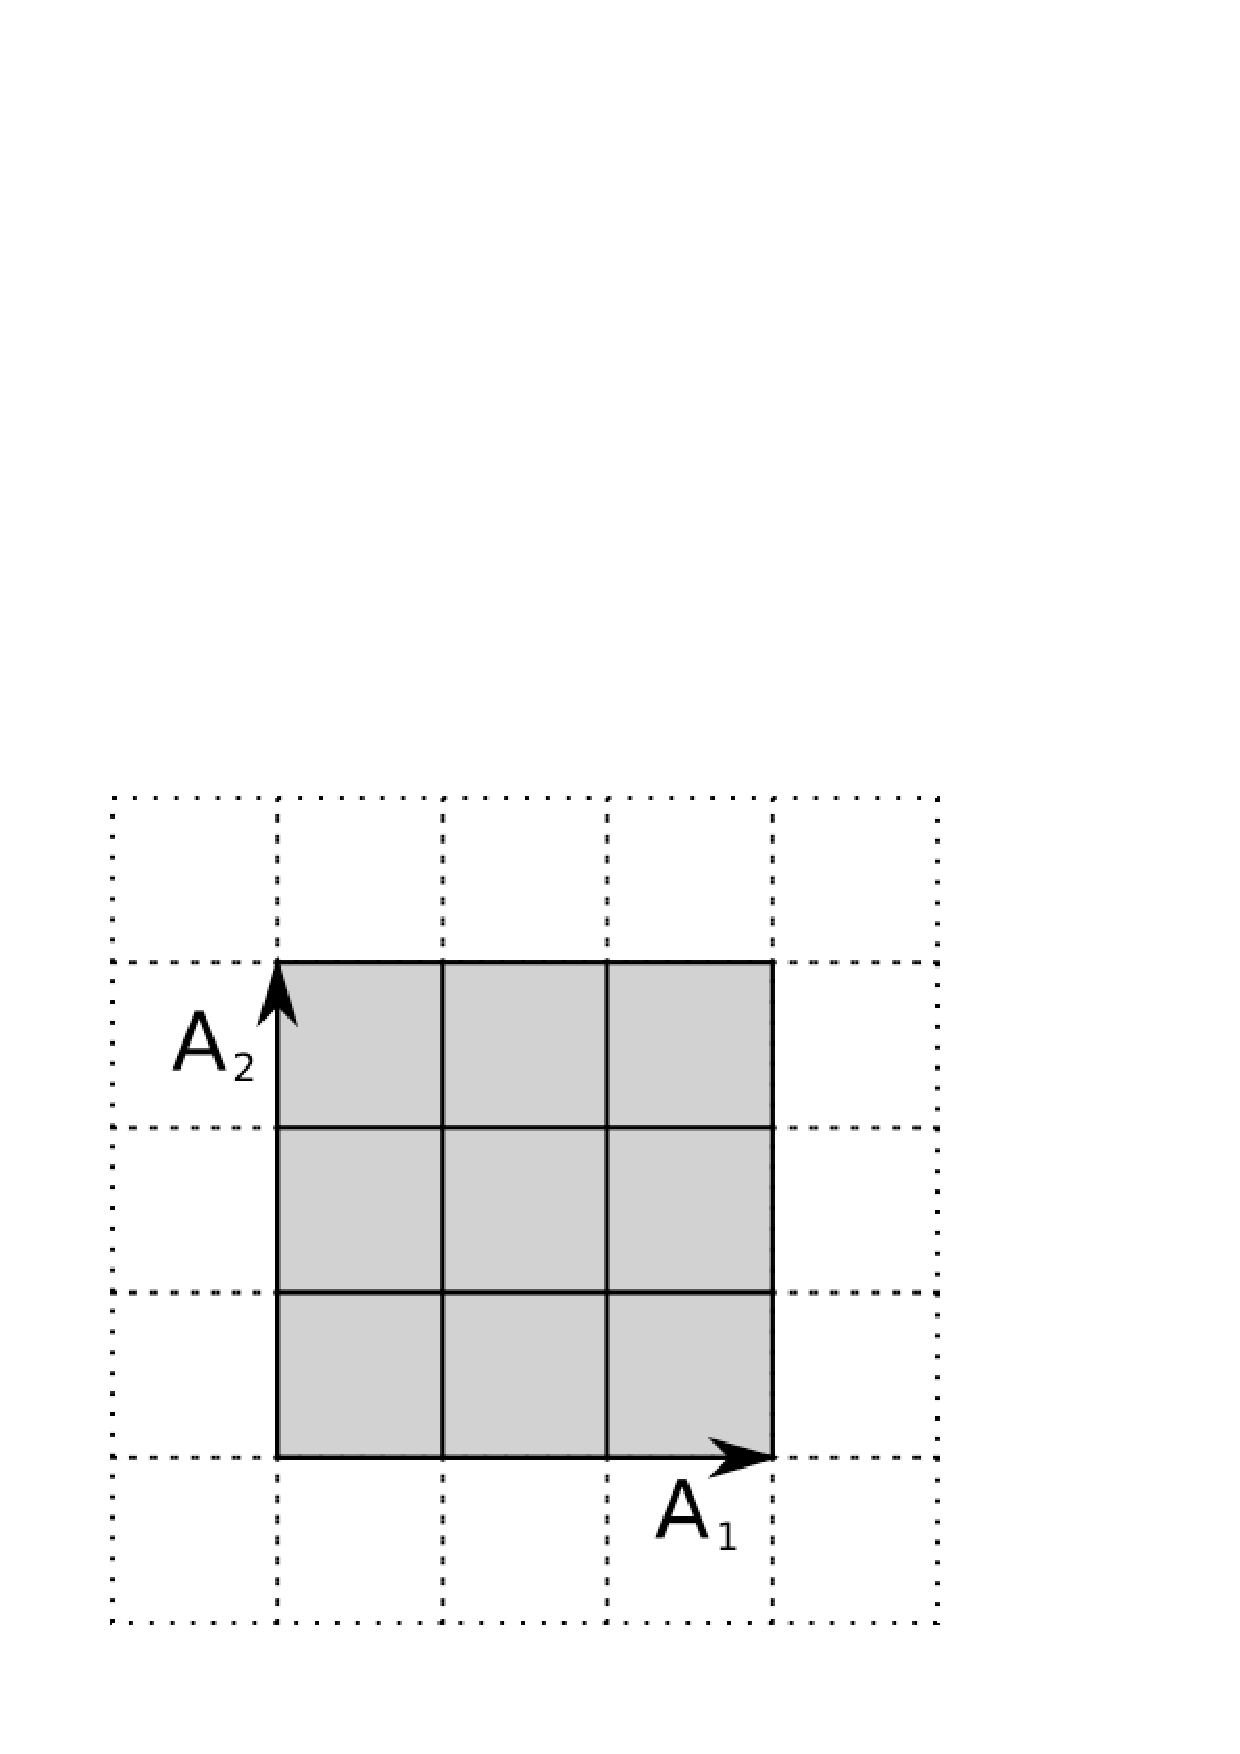
\includegraphics{3x3.pdf}}
\caption{\label{fig:N9} An example of a perfect square packing with density one: $N=9$.}
\end{figure}

There is a more general class of density-one packings, in which the lattice of squares may be tilted with respect to the primitive vectors of the torus. Setting $d=1$ and $c=0$ in Eq. (\ref{eq:gap}), we find $N=n_2^2 + n_4^2$, $n_1=-n_4$, and $n_2 = n_3$, the square lattice being oriented at an angle of $\tan^{-1}(n_2/n_1)$ relative to the torus lattice vectors.   Clearly, these density-one, tilted square lattice solutions are optimal for all $N$ that are sums of two square integers.  Note that the perfect square solution corresponds to the special case $n_2 = n_3 = 0$.  Fig. \ref{fig:bravais} shows the case $N=10$ ($n_1=3$ and $n_2=1$).

\begin{figure}[H]
\scalebox{.4}{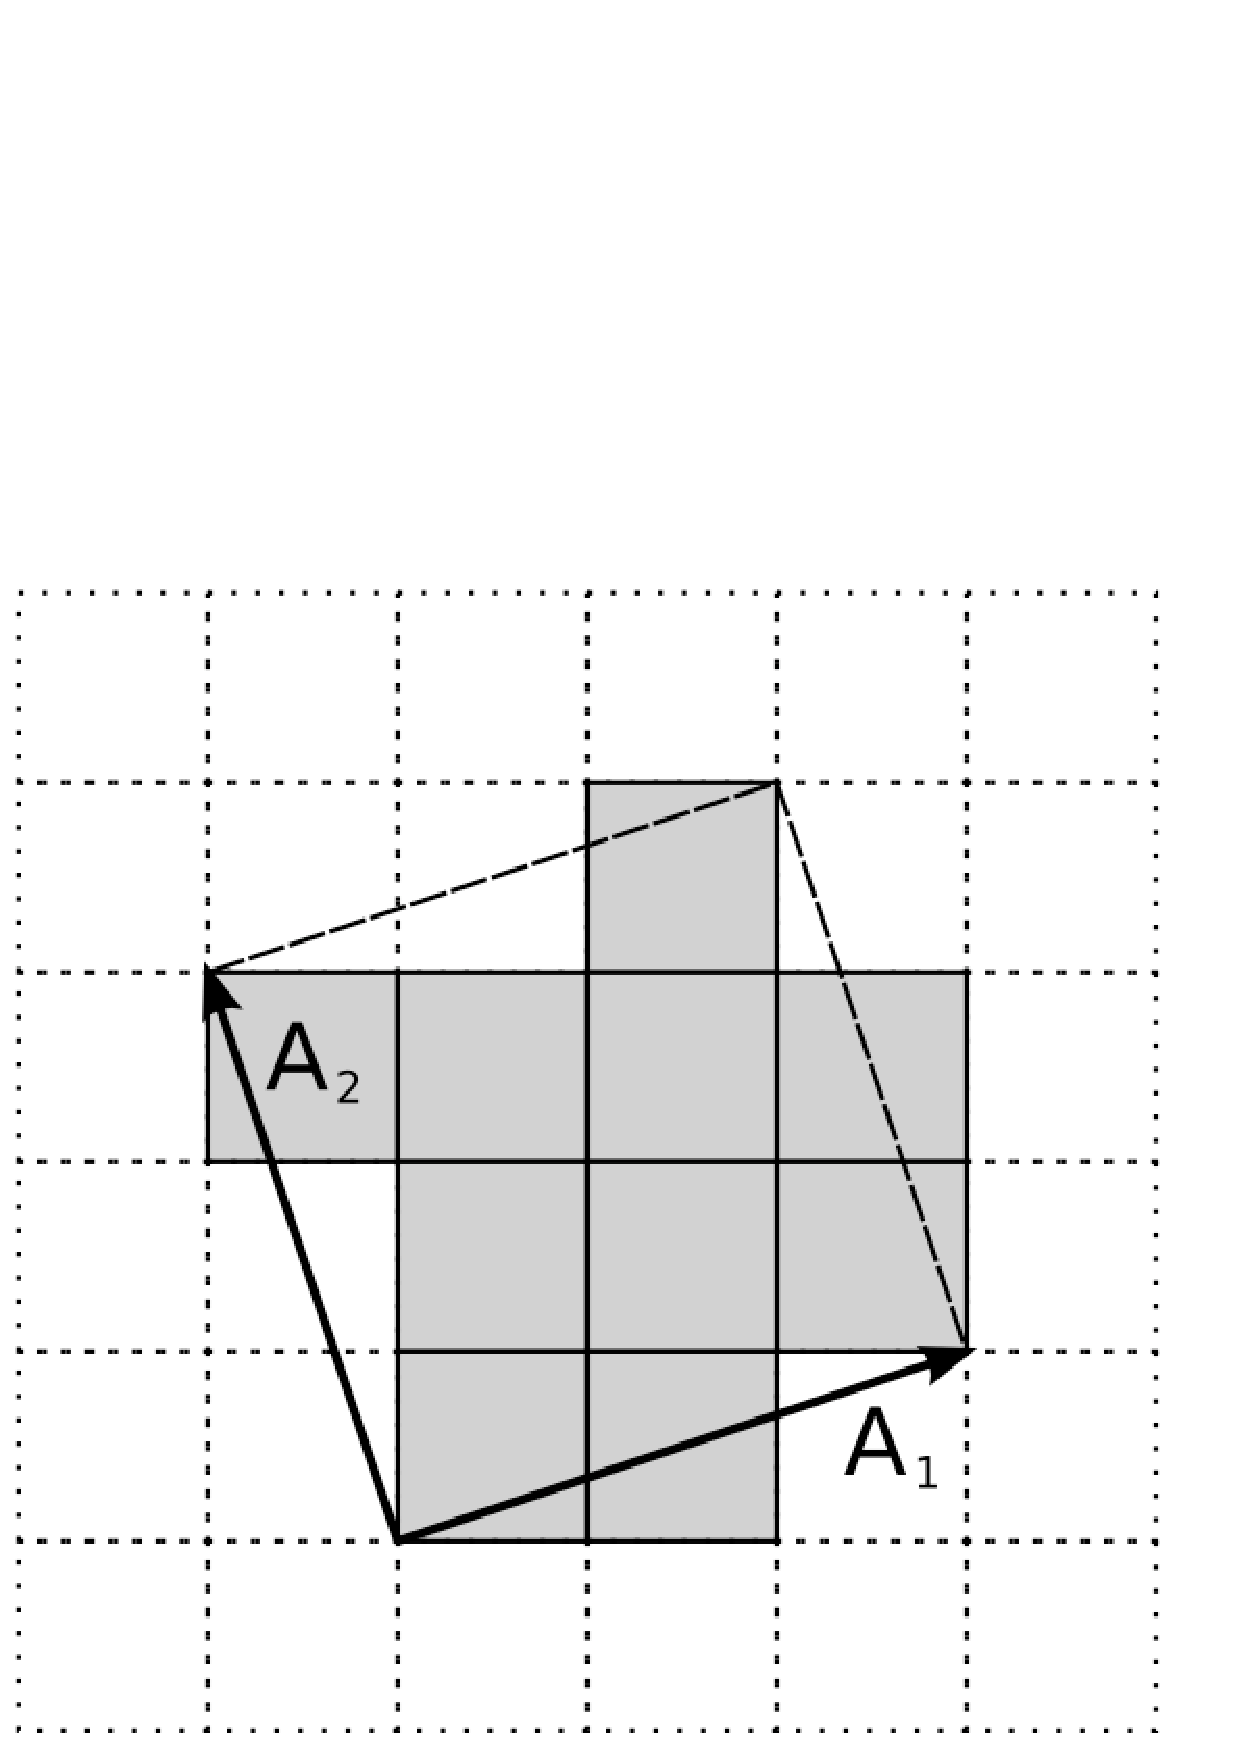
\includegraphics{bravais1.pdf}}
\caption{\label{fig:bravais} An example of a packing for which $N$ is equal to the sum of two squares: $N=10$; all such packings are density one.}
\end{figure}


We thus find that if N is the sum of two squares, there exists a density-one packing. The converse of this is also true: $N$ is a sum of two squares for all density-one packings of squares in the torus. To prove this, first note that every square in a density-one packing must have at least four other squares bordering it along a finite segment length, forcing all $N$ squares to share the same orientation.  Now consider three squares in mutual contact with each other -- a configuration that must exist if the packing has no gaps. Two of those squares must be aligned in a row, as shown in Fig. \ref{fig:aligned}. In order to eliminate gaps in the packing, these three squares define a set of rows that the entire packing must respect. Note that periodic boundary conditions allows us to draw the torus vectors so that they begin on the corner of a square and end on the corresponding corner of another square.  Thus, $n_2$ and $n_4$ are both integers. A right triangle can be constructed with $n_2$ as one side and $A_1$ as its hypotenuse; another right triangle can be drawn with $n_4$ as its base, and $A_2$ as its hypotenuse. (See Fig. \ref{fig:aligned}). These triangles are identical by inspection.  $|A_1|^2$ and $|A_2|^2$ are therfore each equal to $n_2^2 + n_4^2$, via the Pythogorean theorem.

\begin{figure}[H]
\scalebox{.4}{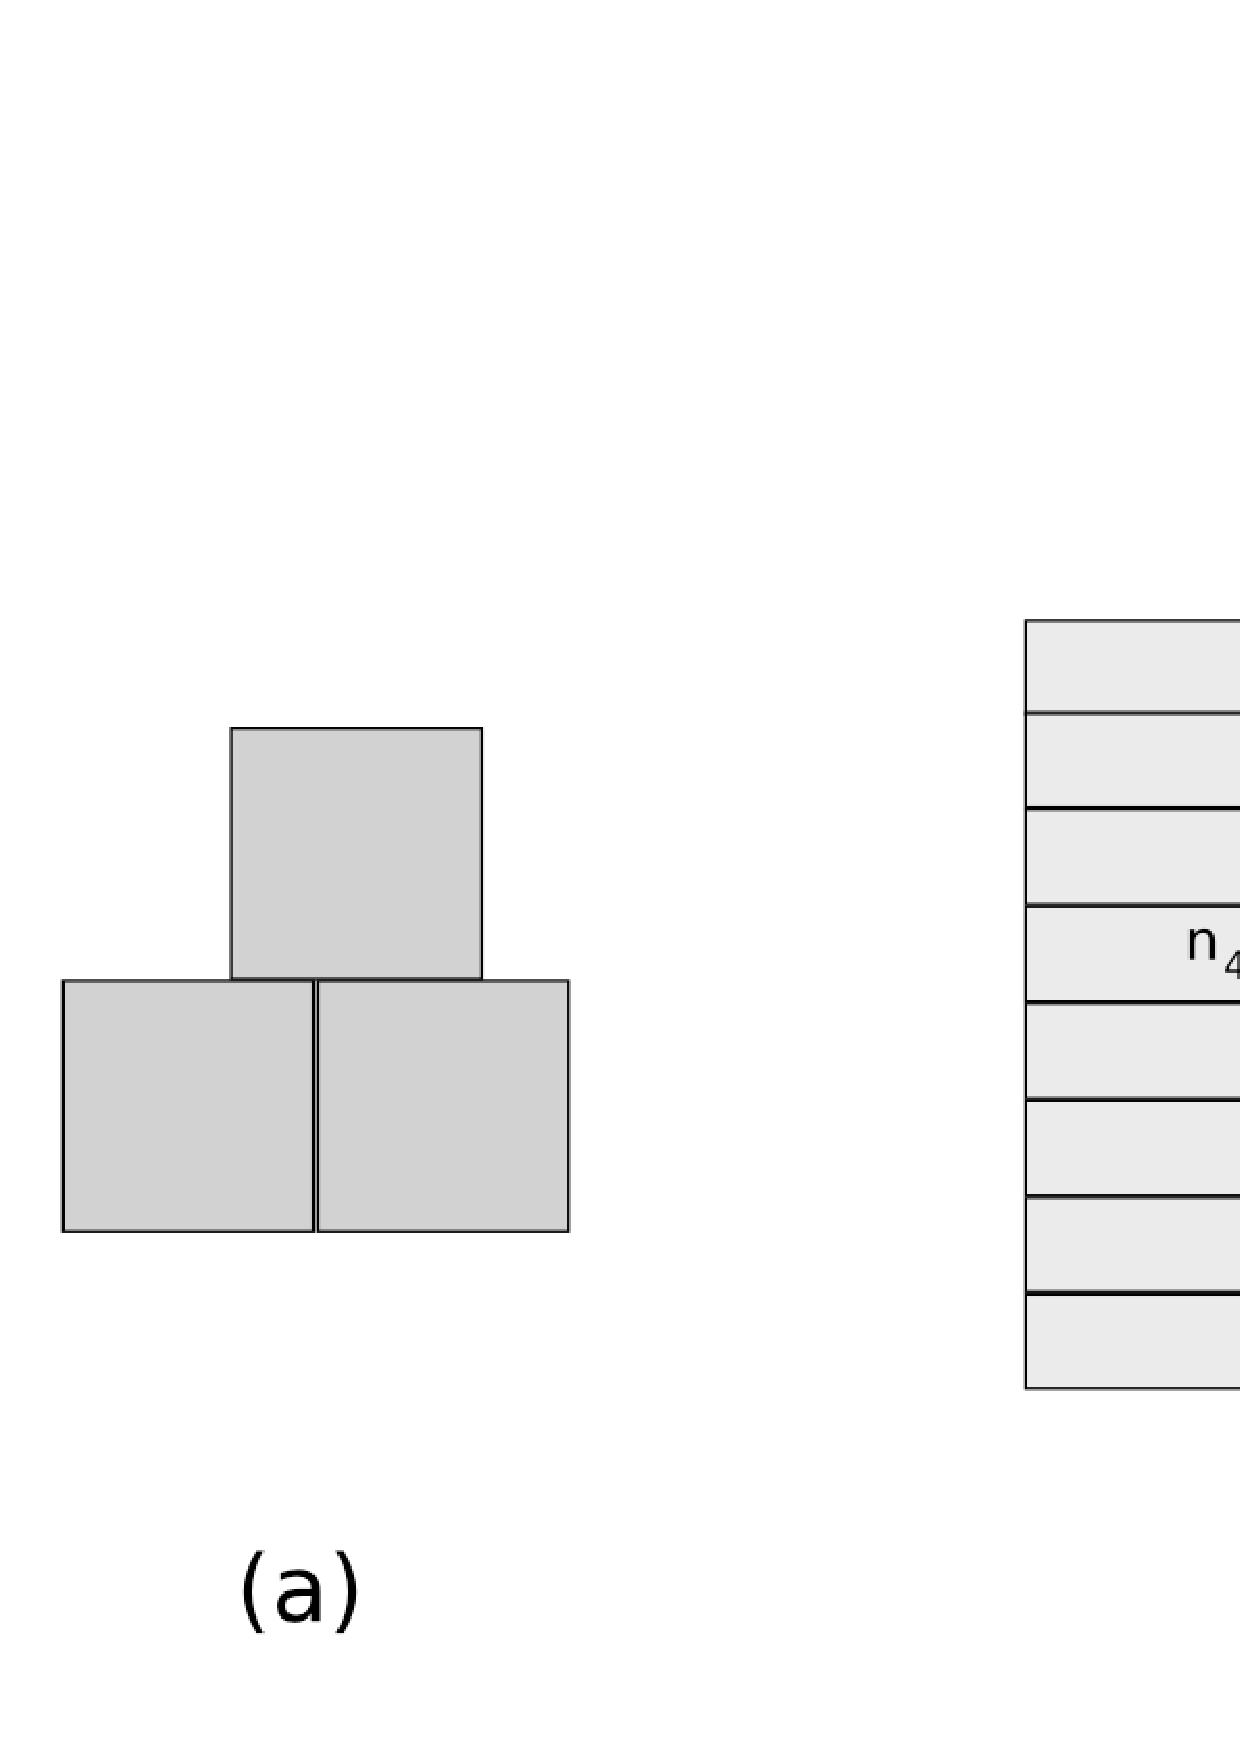
\includegraphics{alignedBlocks3.pdf}}
\caption{\label{fig:aligned} (a) Any three squares in mutual contact without gaps force two of the squares to define a row. (b) Diagram illustrating that $N$ must be equal to the sum of two squares for all density-one packings of squares in the torus (see discussion in section \ref{sec:densityOnePackings}).}
\end{figure} 

\subsubsection{Lattice packings with vacancies}
\label{sec:vacancies}
The simplest way to produce candidates for a densest packing for $N=n_2^2 + n_4^2-k$ is to remove $k$ squares from a density-one packing; indeed, our numerical results suggest that for several values of $N$, the densest packing is a density-one packing with one missing square.  This is indicated in the Comment column in the Table using the notation $n_1^2-1$ or $n_1^2+ n_2^2-1$, depending on whether they are generated by removing $1$ square from $N$ a square integer, or a sum of two square integers respectively.  As is demonstrated in Fig. \ref{fig:n7} for the case of $N=2^2+2^2-1=7$, such vacancies allow for continuous displacement of other squares within a row, leading to a finite entropy for such configurations.  Other examples include $N=3$ and $15$.

\begin{figure}[H]
\scalebox{.48}{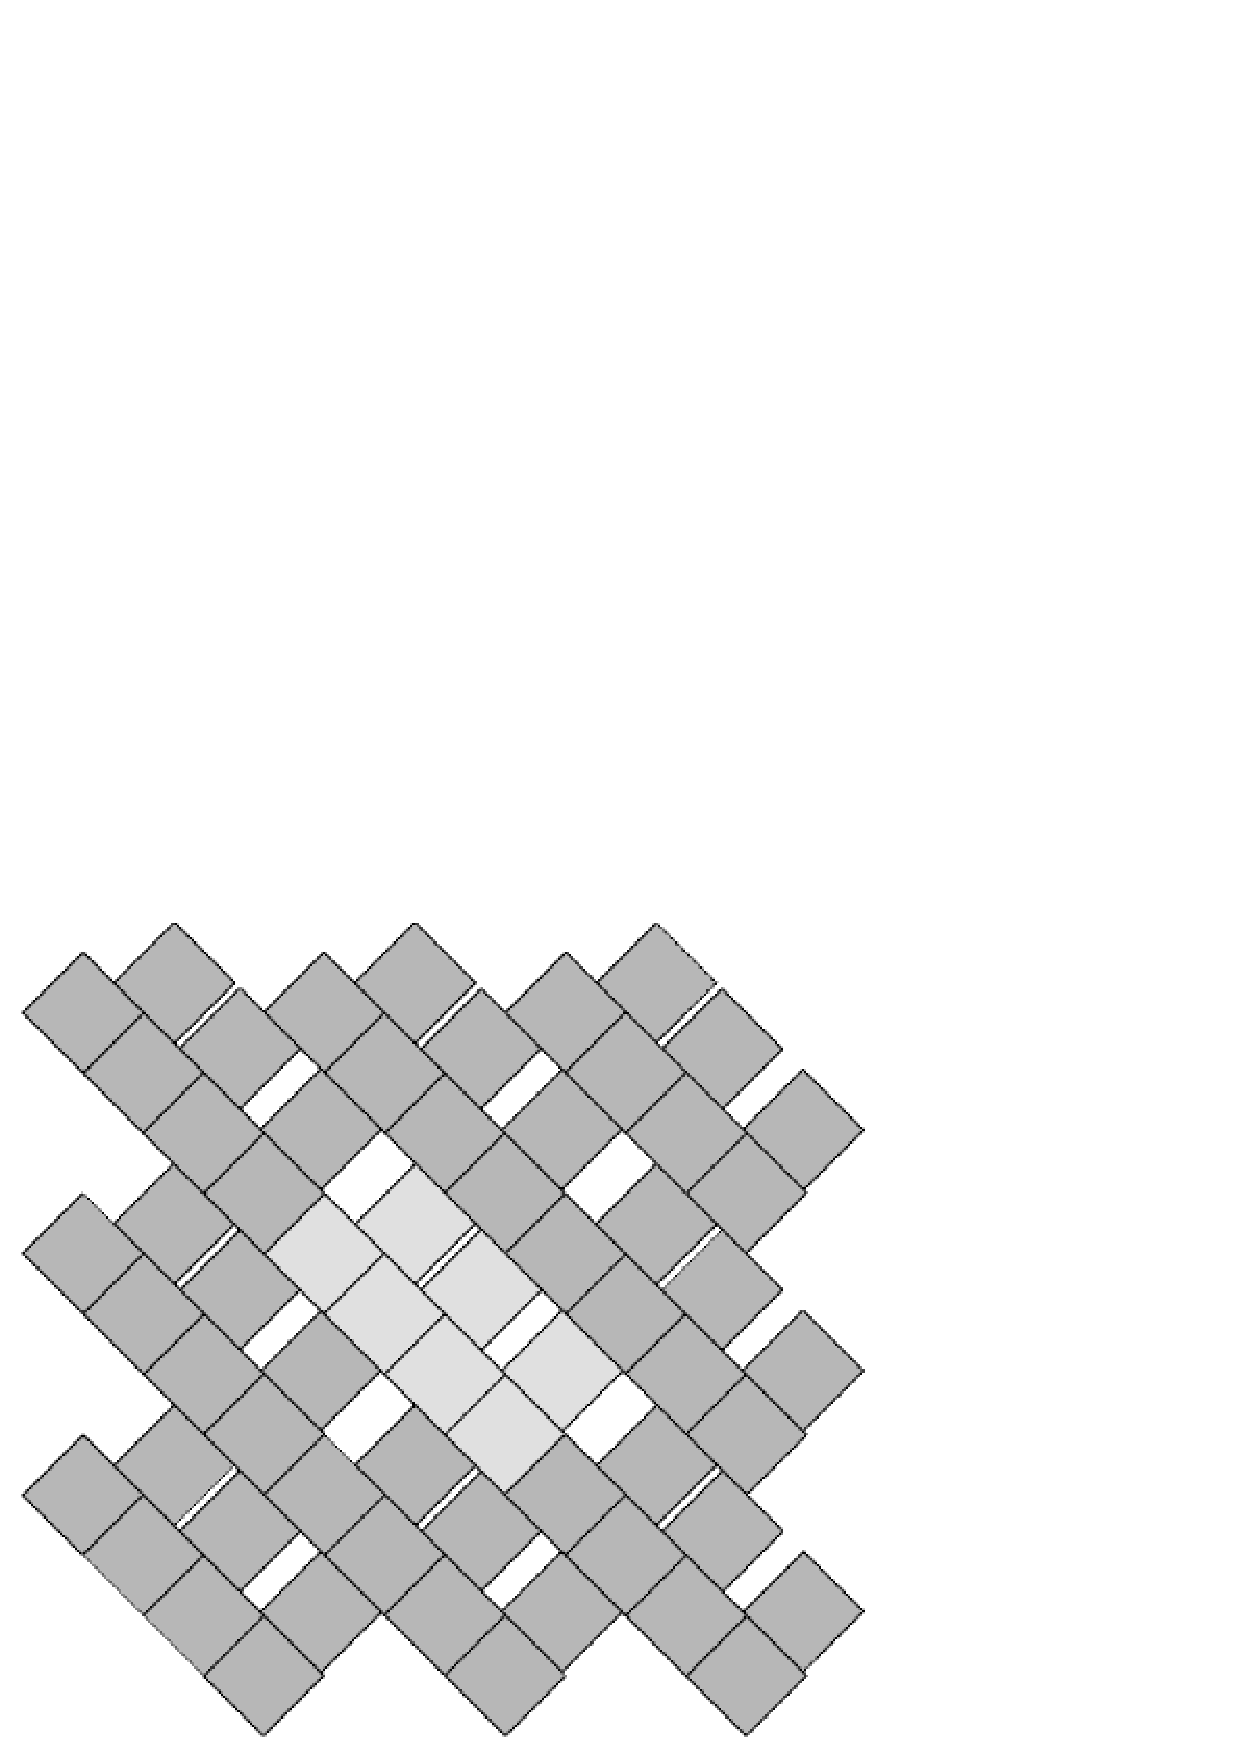
\includegraphics{n7a.pdf}}
\caption{\label{fig:n7} An example of a packing with vacancies with the form $N=n_2^2 + n_4^2-k$. Here $N=7, k=1$ and $n_2=n_4=2$.}
\end{figure}

\subsubsection{Bricklayer packings with gaps}
\label{sec:bricklayer}
Next we consider Bravais lattice solutions that have density less than one -- that is, packings with gap $d-1 > 0$.  Because these solutions have rows that are shifted relative to one another ($c\neq 0$), we call these ``gapped bricklayer configurations.''  An example is shown in Fig. \ref{fig:gb}(a).  Equations (\ref{eq:gap}) allow us to ennumerate all gapped bricklayer configurations. Since the packing density of these configurations is $(n_2^2 + n_4^2)/N$, the highest packing density we can find within this class of configurations with density less than unity must have the form $n_2^2 + n_4^2 = N-1$.  This requires that $N$ be one more than a sum of two squares. The first several are gapped bricklayer configurations are seen for $N=$ 2,3,6,11,14,18,26, and 27.  Based on the numerics we believe that for $N=6$, 11, 14 and 27, the gapped bricklayer packing is the densest possible packing. These are indicated in the Table with the abbreviation ``GB'' in the Comment column. Associated (non-unique) lattice vectors are shown in the rightmost columns of the Table for the GB packings.  There are also gapped bricklayer solutions for density $(N-2)/N$ when $N$ is two more than a sum of two squares, though we have not found any candidate densest packing solutions of this form for $N \leq 27$. Unlike the bravais lattice packings with density one, different rows of the gapped bricklayer solutions have a fixed shift given by $c = - (n_1 n_2 + n_3 n_4)/(n_2^2 + n_4^2)$, where the denominator is the closest sum of two squares below $N$. 

\begin{figure}[H]
\scalebox{.48}{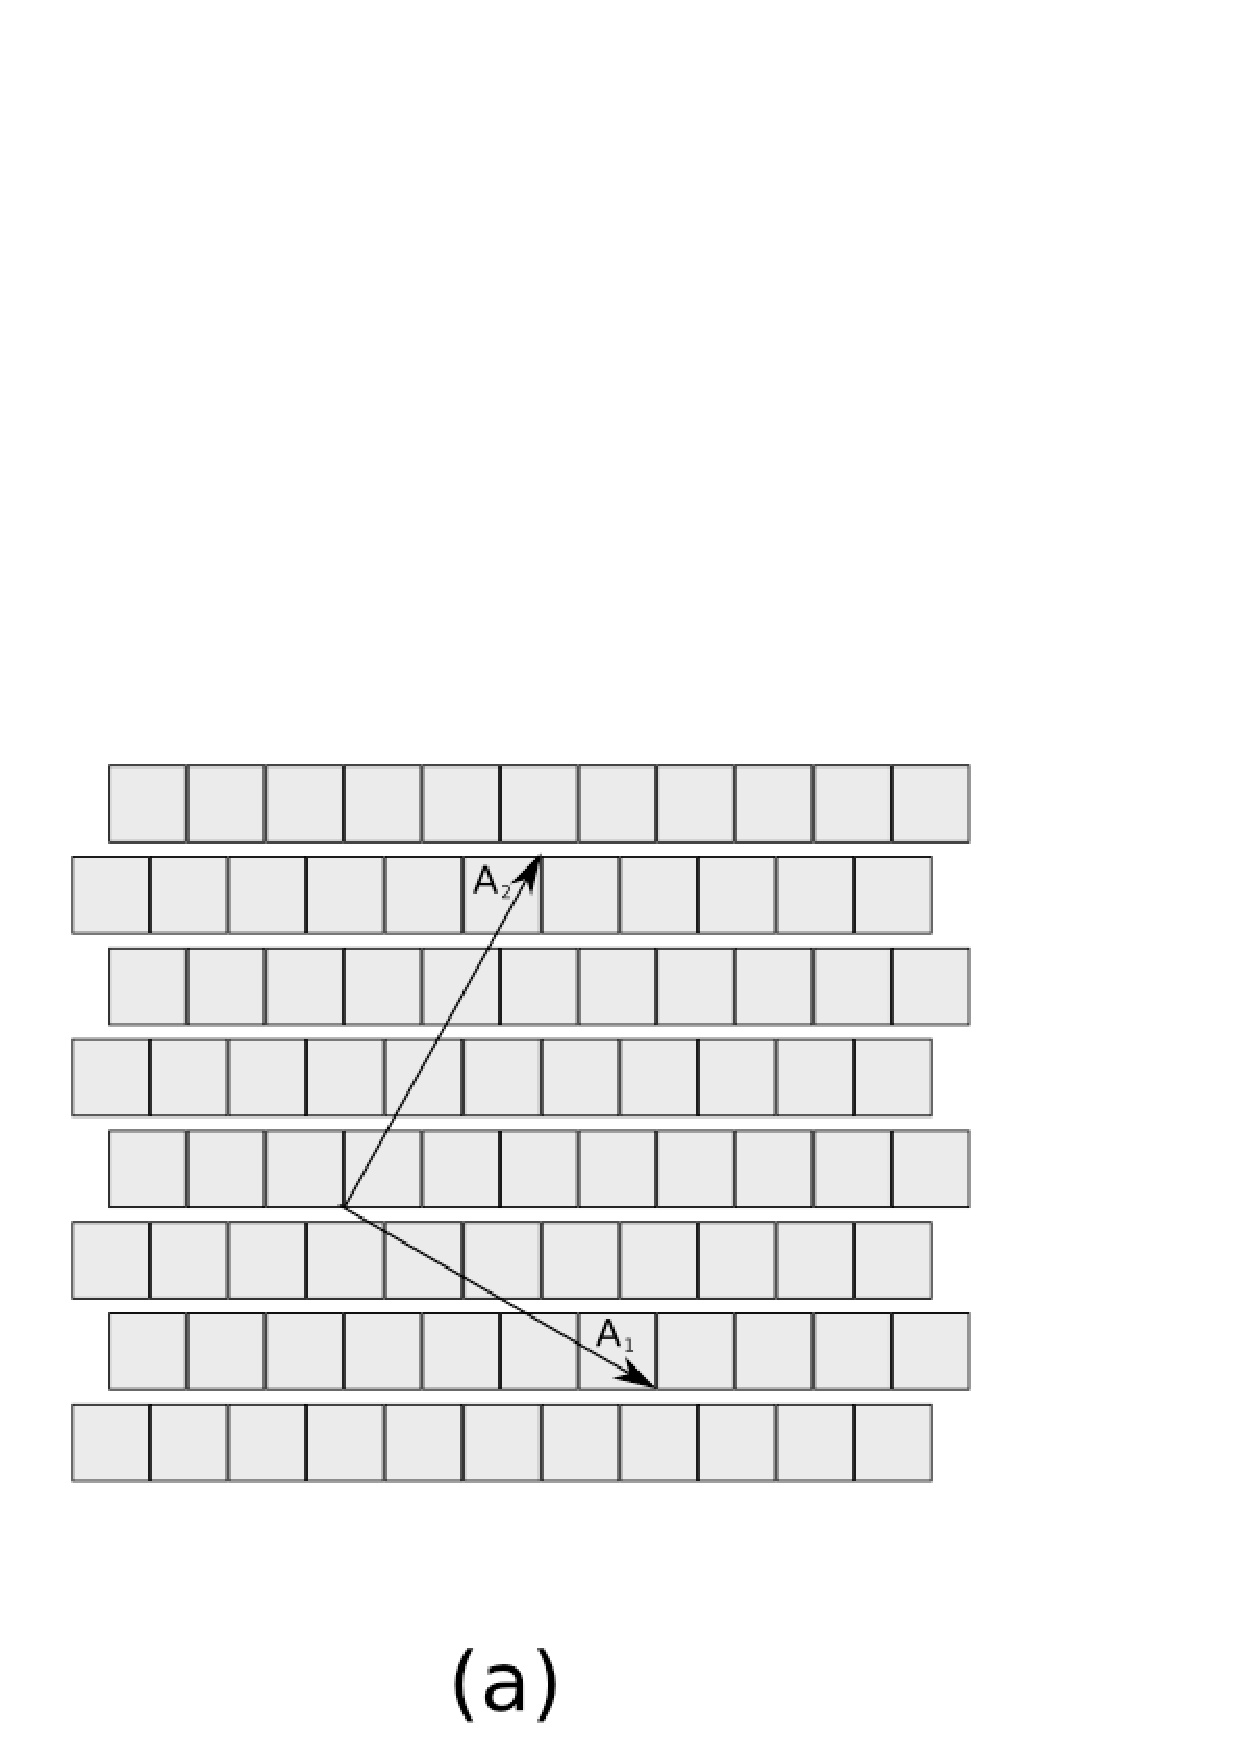
\includegraphics{gappedCombo1.pdf}}
\caption{\label{fig:gb}Schematic (a) of a ``gapped bricklayer'' configuration, with density $\rho = (N-1)/N$. Results of simulated annealing for $N=11$ are shown in (b) ($n_1=3, n_2=1, n_3=-2, n_4=3$).  The finite entropy of this configuration is revealed by the displacements of the squares perpendicular to the rows.}
\end{figure}


\subsection{Non-Bravais Lattice Packings}

Here, we consider special cases suggested by our numerical simulations that do not correspond to Bravais lattice packings.
Note: if the Comment column of the Table simply repeats a value of $N$, it indicates a special case for which the squares are not on a Bravais lattice and for which there is not an obvious pattern that can be extrapolated easily to optimal packings for higher values of $N$.

\subsubsection{Gapped bricklayer with domino bricks, $N=22$}
The conjectured best packing for $N=22$ is shown in Fig. \ref{fig:n22}. This packing is in fact a gapped bricklayer configuration, except that the unit cell or brick is composed of two squares stacked in the $\hat{{\bf y}}$ direction (the direction perpendicular to the rows).  The configuration is otherwise identical to the $N=11$ gapped bricklayer and has density $\rho= 10/11$.

\begin{figure}[H]
\scalebox{.7}{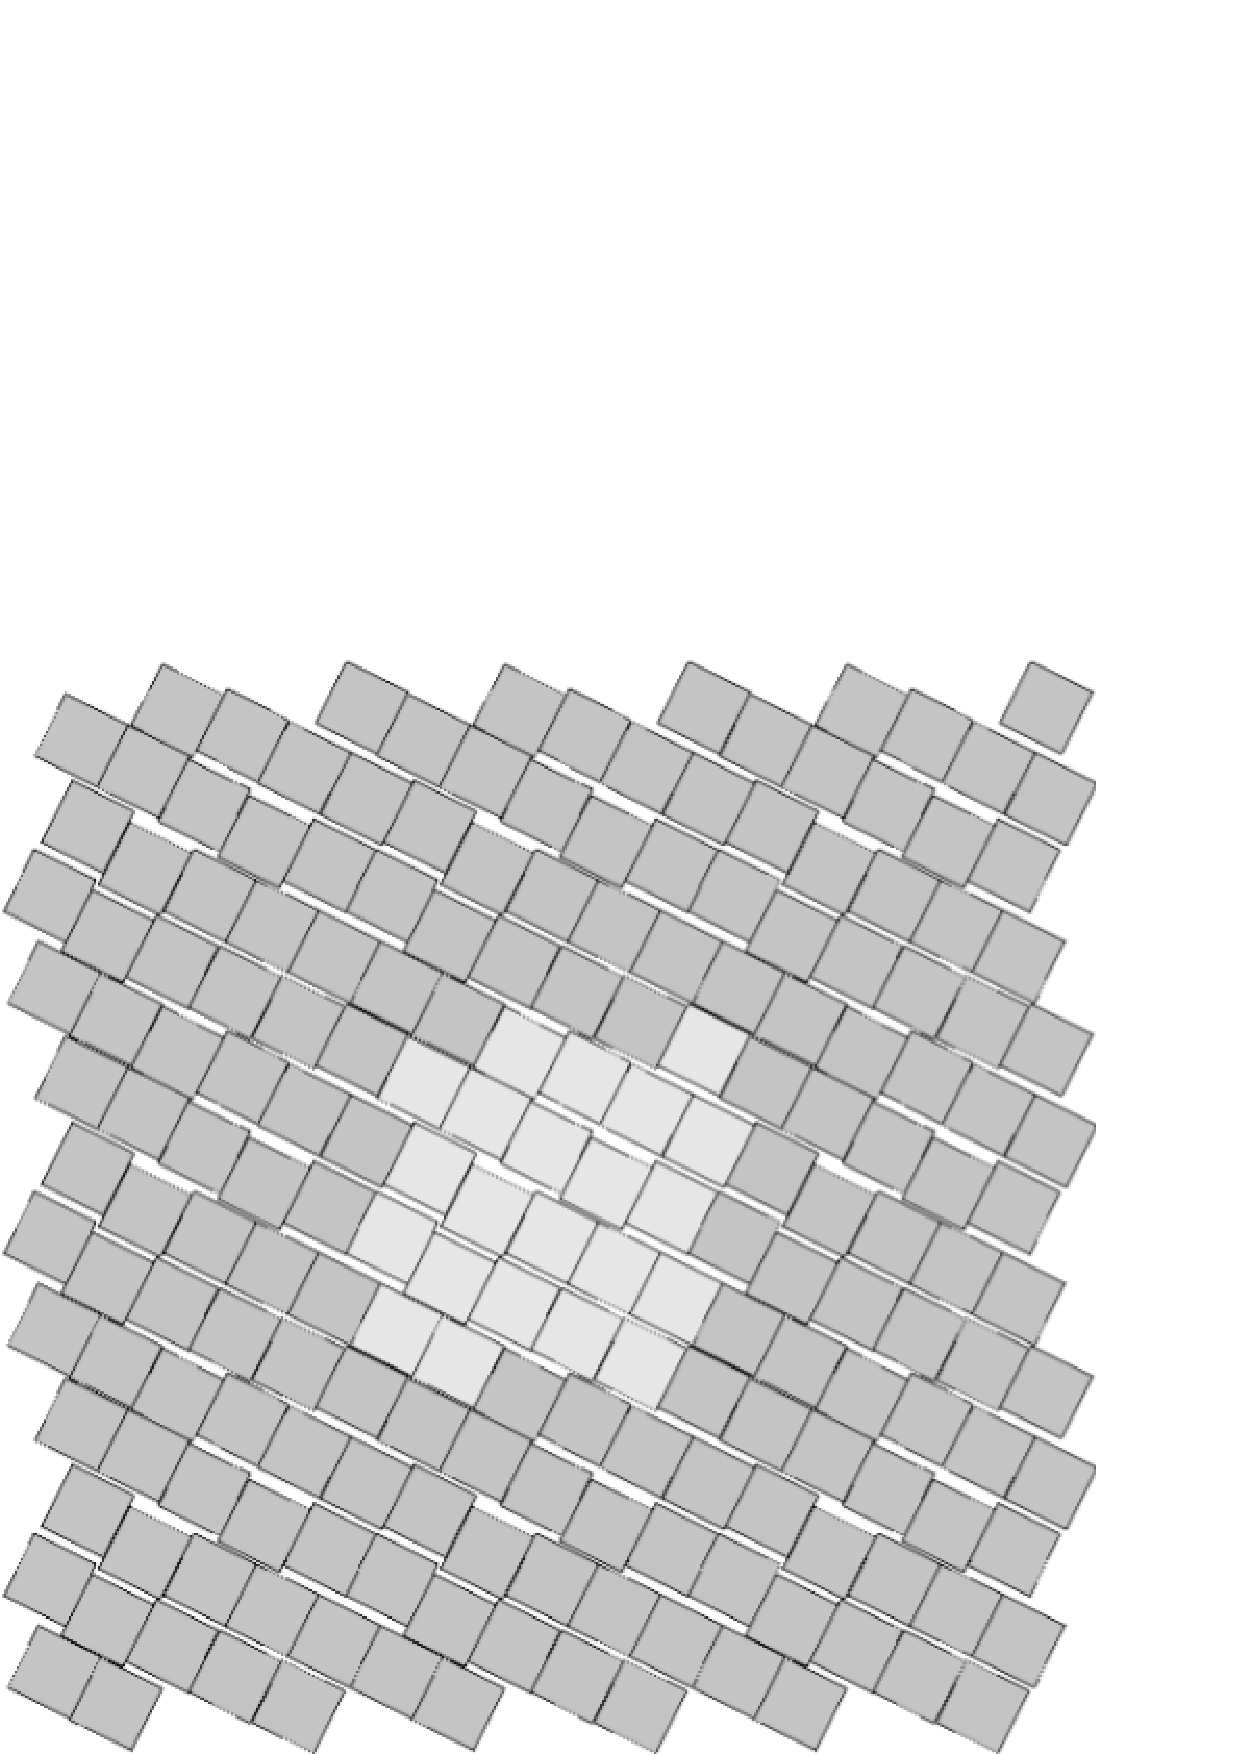
\includegraphics{n22Edit.pdf}}
\caption{\label{fig:n22}Simulation results for $N=22$: the conjectured best packing is a ``gapped bricklayer with domino bricks''.}
\end{figure}

\subsubsection{Lattice of $\frac{1}{2}\times\frac{1}{2}$ holes, $N=12$ and $23$}
The conjectured best configurations for $N=12$ and 23 are shown in Figs.\ \ref{fig:n12} and \ref{fig:n23}, respectively.  In both cases the motif can be described as a lattice of $\frac{1}{2}\times\frac{1}{2}$ holes.  The torus lattice vectors, Eq.\ \ref{eqn:Ana} with $\ax=\hat{{\bf x}}$ and $\ay=\hat{{\bf y}}$, for $N=12$ are described by $n_1=n_2=-n_3=n_4=5/2$ and the torus lattice vectors for $N=23$ are described by $n_1=n_4=9/2$, and $-n_2=n_3=2$.  It is straightforward to verify that these motifs are in fact packings on the torus and have the density $N/(n_2^2 + n_4^2)=N/(N+k/4)$ where $k$ is the number of holes in the unit cell.  For $N=12$, evidently $k=2$ and for $N=23$, $k=5$. 

\begin{figure}[H]
\scalebox{.7}{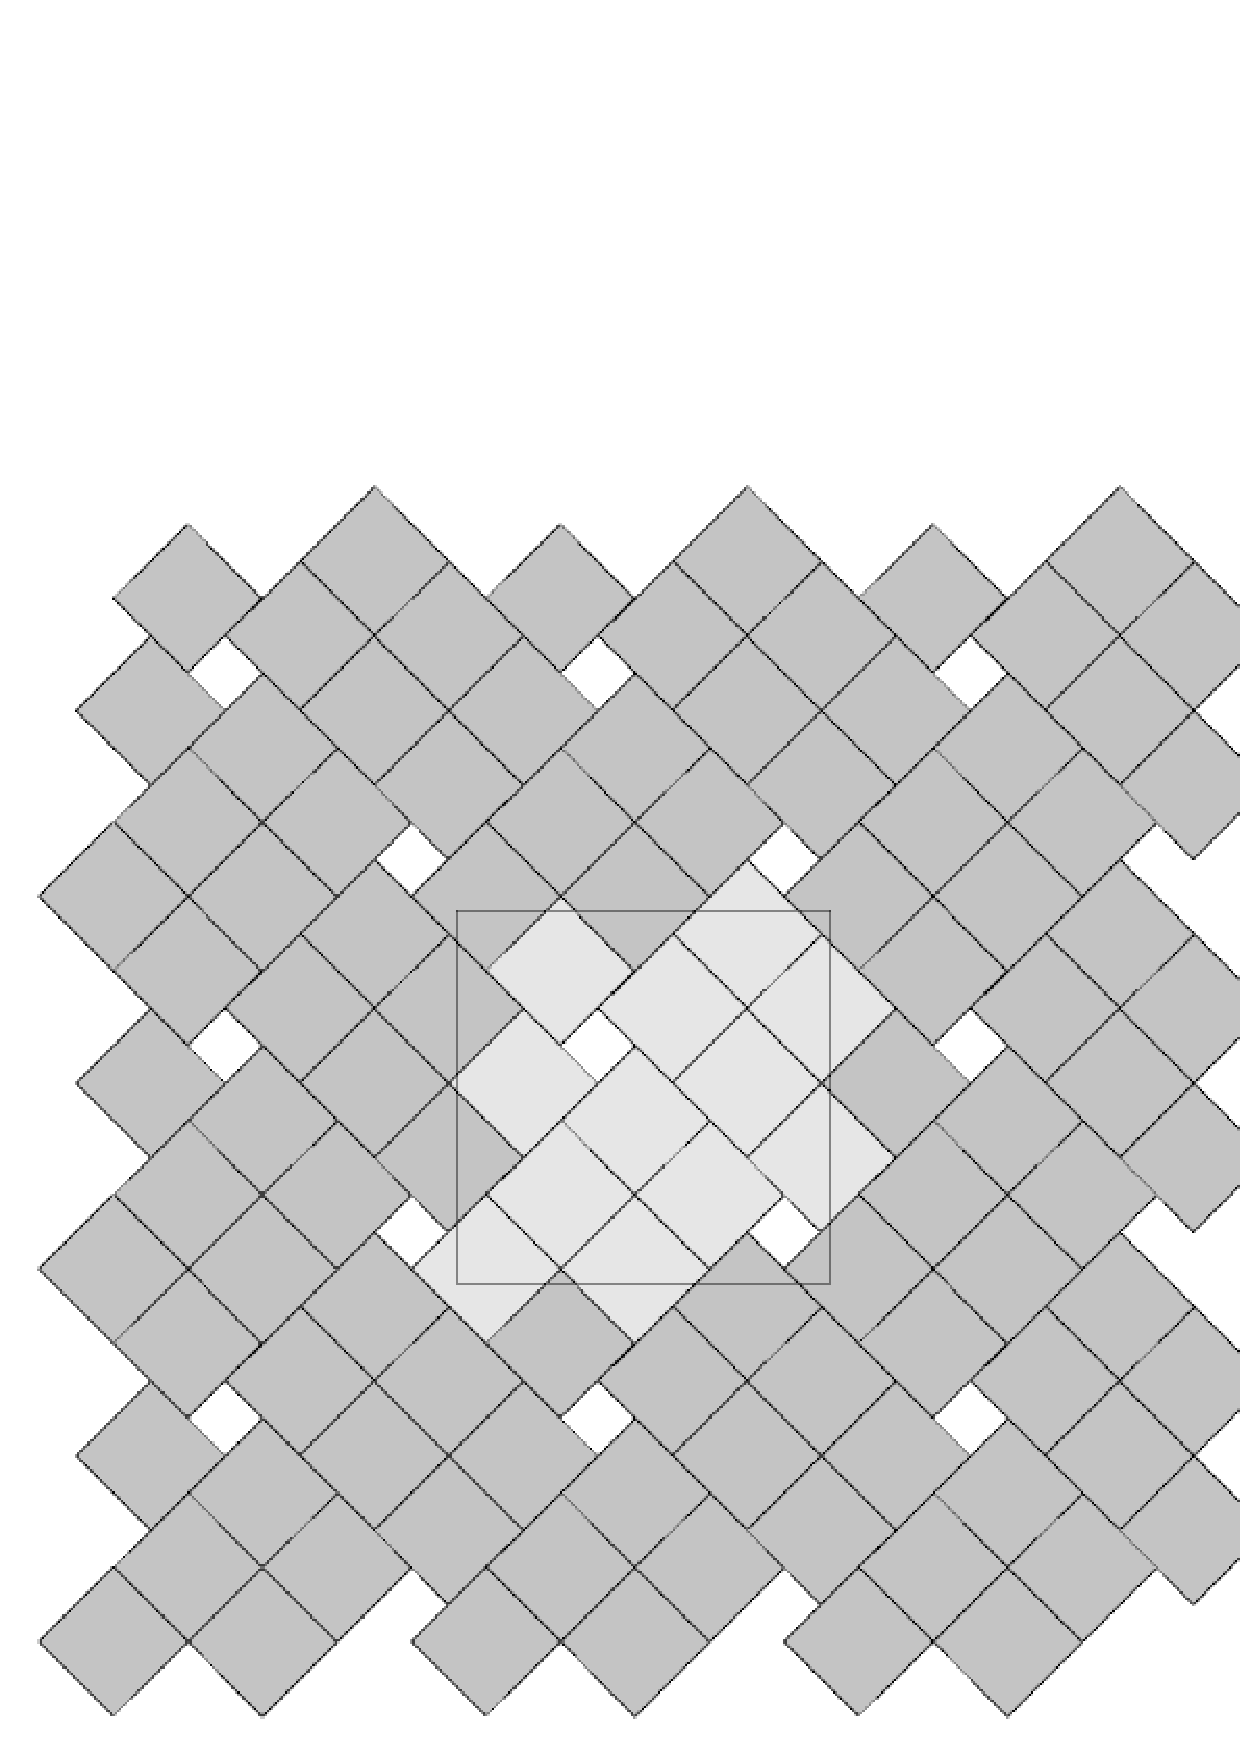
\includegraphics{n12edit.pdf}}
\caption{\label{fig:n12}Simulation results for $N=12$: a lattice of $\frac{1}{2} \times \frac{1}{2}$ holes.}
\end{figure}

\begin{figure}[H]
\scalebox{.5}{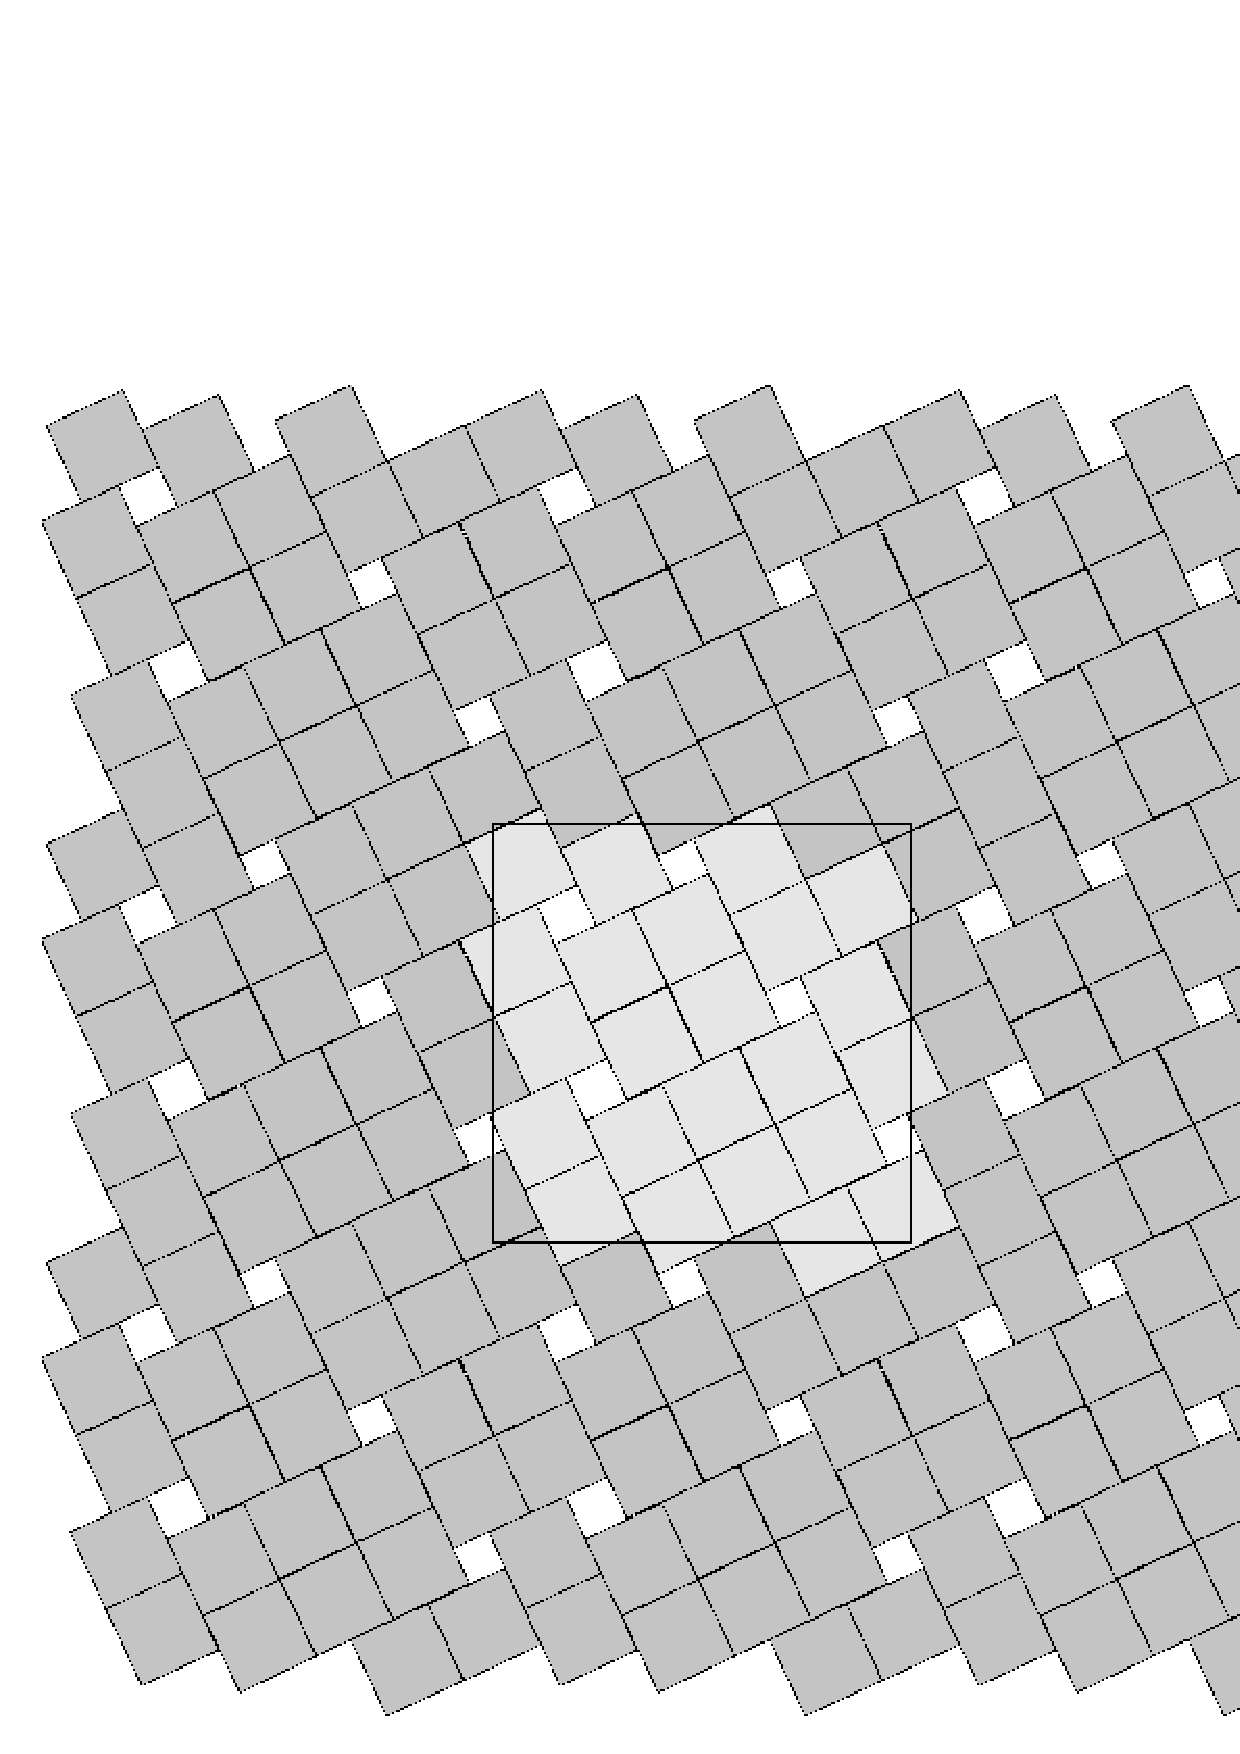
\includegraphics{N23.pdf}}
\caption{\label{fig:n23}Simulation results for $N=23$: a lattice of $\frac{1}{2} \times \frac{1}{2}$ holes.}
\end{figure}




\subsubsection{Lattice of skew squares embedded in a square lattice, $N=21$}
The conjectured densest packing for  $N=21$, shown in Fig.\ \ref{fig:n21}, does not follow any of the motifs described heretofore. The unit cell consists of a $4 \times 4$ square with motif of 5 squares attached to its side.  This 5-square pattern is also the best packing of 5 squares in a square \cite{Friedman2002}.  A simple calculation yields the density, $\rho= 21/(4^2+(2+1/\sqrt{2})^2)$. This packing has one square per unit cell tilted at 45$^{\circ}$ relative to all other squares.  This is the only example that we found for which not all of the squares in the motif are oriented in the same way. It was also the most difficult configuration for our simulated annealing algorithm to find. Figure \ref{fig:n21} shows a typical simulation result, which clearly has not yet fully converged.

\begin{figure}[H]
\scalebox{.4}{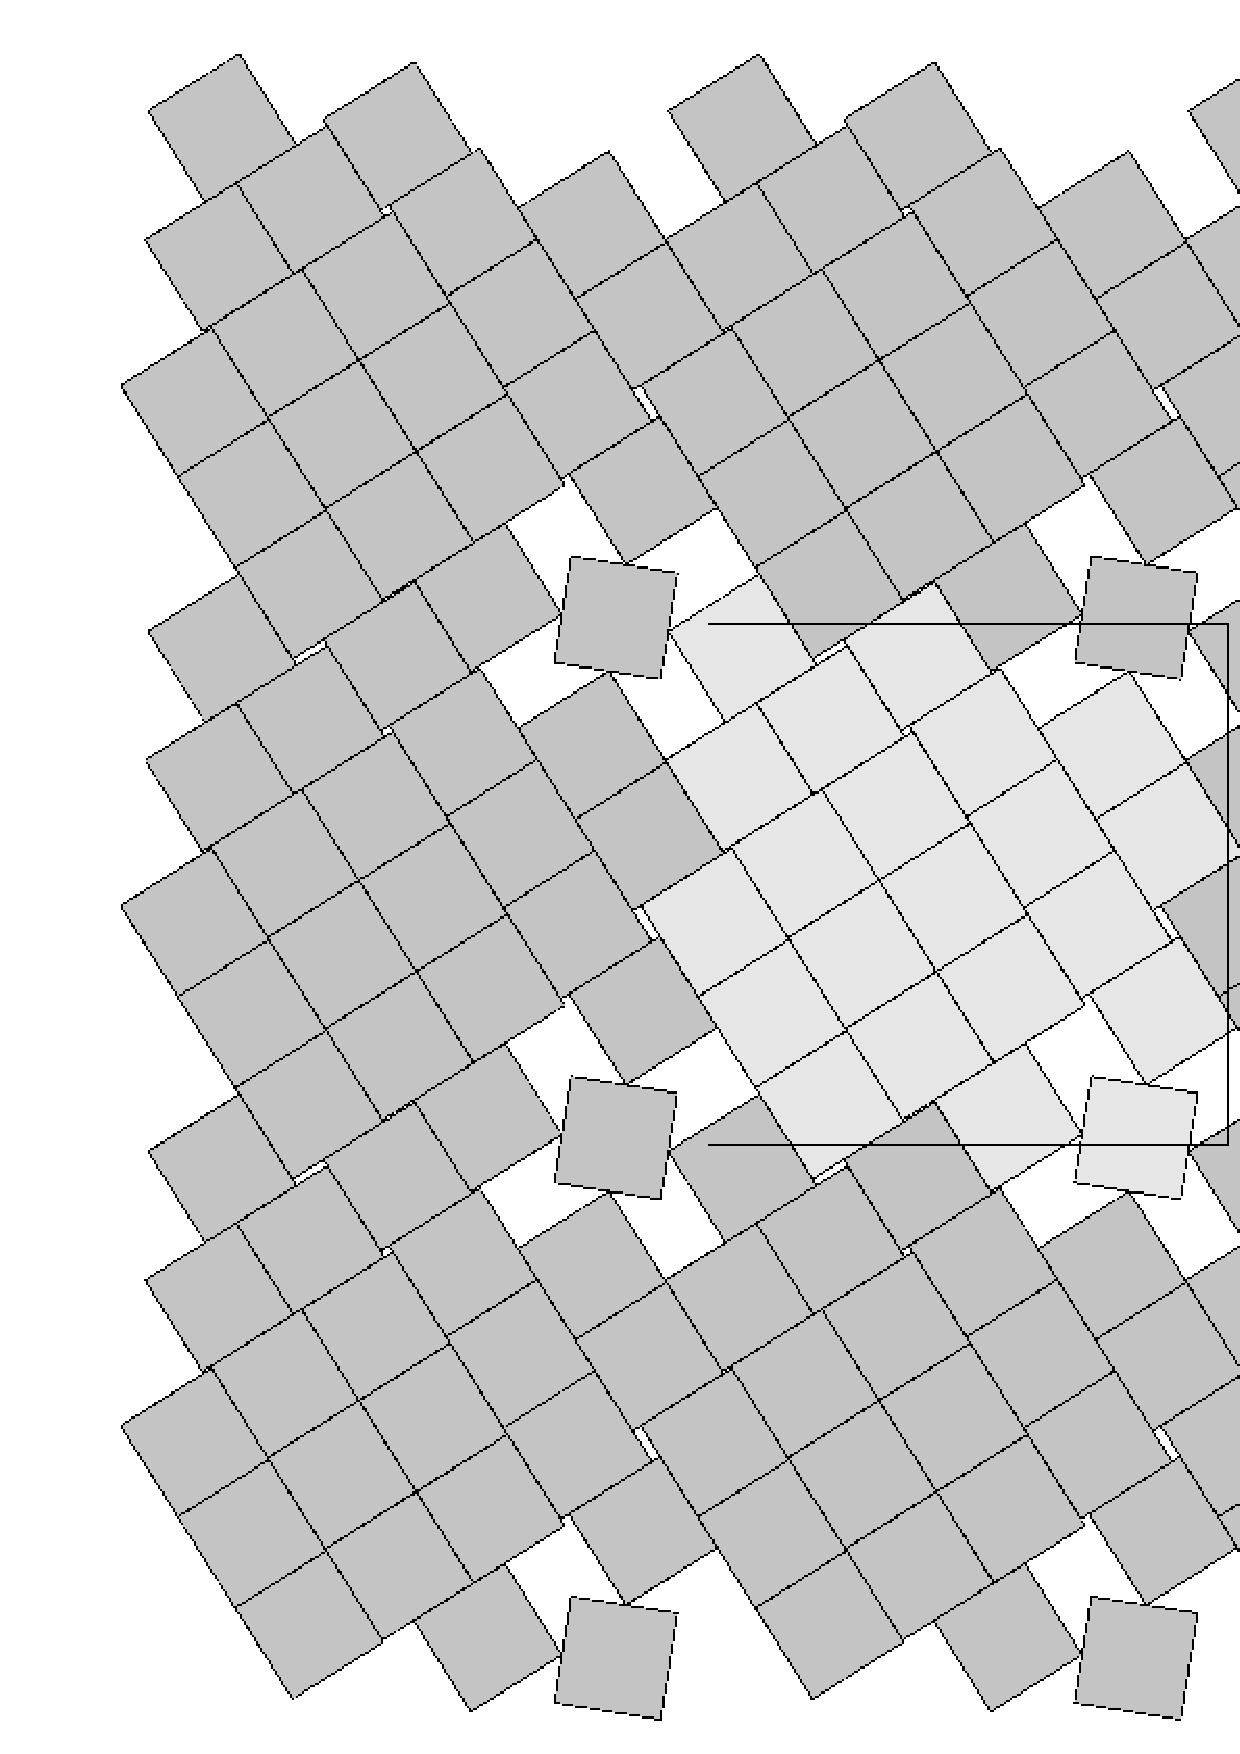
\includegraphics{N21.pdf}}
\caption{\label{fig:n21}Simulation results for $N=21$: a lattice of skew squares embedded in a square lattice.  The $5$-square pattern (which includes a skew square in its center) is the proved best packing of 5 squares in a square \cite{Friedman2002}. Note that the simulation results have not yet converged to the conjectured best packing.} \end{figure}


\subsection{Table of Results}

To summarize: the perfect square, sum of two squares and gapped bricklayer configurations cover most of the case we have found for $N \leq 27$.  The Table gives densest packing configurations (if $\rho=1$) and conjectured densest packing configurations (if $\rho<1$), for each value of  $N$ less than 28.  The column ``$\rho$'' is the density of the configuration. The Comment column describes the type of lattice.   For example, $3^2$ indicates a perfect square and $5^2-1$ indicates a perfect square with one square missing.  Similarly $3^2+1^2$ refers to the sum of two squares and ``GB'' stands for ``gapped bricklayer.''  If a single number is in the Comment column it refers to one of the special cases discussed above.  The four columns ``$n_1$, $n_2$, $n_3$, $n_4$'' are shown if the configuration of squares is itself a Bravais lattice; these integers are the coefficients of the lattice vectors of the torus, in terms of the lattice vectors of the squares as defined in Eq. (\ref{eqn:Ana}).  Only those columns needed to specify the lattice are filled in.

\vspace{.3in}
\begin{table}
\label{table}
\caption{Exact and conjectured densest packed configurations of squares on a torus.  Refer to the text for the meaning of the columns.}
  \begin{tabular}{|c | c|c | c| c | r | c | c | c |}
\hline
  $N$ &$\rho$&Comment& $n_1$ & $n_2$ & $n_3$ & $n_4$  \\ \hline \hline
   1 &1&  $1^2$ & 1&  &   &    \\ \hline 
   2 &1&  $1^2+1^2$ &1& 1 &  &  \\ \hline
   3 &$3/4=0.75$&  $2^2 -1$ &2&  & &   \\ \hline
   4 &1&  $2^2$ &2& & &   \\ \hline
   5 &1&  $2^2+1^2$ &2& 1 &    & \\ \hline
   6 &$5/6=0.8\bar{3}$& GB &2& -1 &2 & 2   \\ \hline
   7 &$7/8=0.875$& $2^2+2^2 -1$ &2& 2 & &     \\ \hline
   8 &1& $2^2+2^2 $ &2& 2 & &     \\ \hline
   9 &1&  $3^2$ &3& & &  \\ \hline
   10 &1&  $3^2+1^2$ &3& 1 &    & \\ \hline
   11 &$10/11=0.\overline{90}$& GB &3& 1 &-2 & 3   \\ \hline
   12 &$24/25=0.96$& 12 && & &    \\ \hline
   13 &1&  $3^2+2^2$ &3& 2 &    & \\ \hline
   14 &$13/14=0.9\overline{285714}$& GB &4& -2 &1 & 3   \\ \hline
   15 &$15/16=0.9375$&  $4^2 -1$ &4&  & &   \\ \hline
   16 &1&  $4^2$ &4& & &   \\ \hline
   17 &1&  $4^2+1^2$ &4& 1 &    & \\ \hline
   18 &1&  $3^2+3^2$ &3& 3 &    & \\ \hline
   19 &$19/20=0.95$&  $4^2 +2^2 -1$ &4& 2 & &   \\ \hline
   20 &1&  $4^2+2^2$ &4& 2 &    & \\ \hline
   21 &$21/(4^2+(2+1/\sqrt{2})^2)=0.900189 \ldots$&  $21$ & &  &   &    \\ \hline 
   22 &$10/11=0.\overline{90}$& 22 &3& 1 &-2 & 3  \\ \hline
   23 &$92/97=0.94845 \ldots$&  $23$ & &  &   &    \\ \hline
   24 &$24/25=0.96$&  $5^2 -1$ &5&  & &   \\ \hline
   25 &$1$&  $5^2$ &5&  & &   \\ \hline
   26 &1&  $5^2+1^2$ &5& 1 &    & \\ \hline
   27 &$26/27=0.\overline{962}$& GB &5&1 &-2 & 5  \\ \hline

\hline
\end{tabular}
\end{table}

\section{Numerical Methods}
\label{sec:numerical}

For all $N \leq 27$ squares on the flat torus, we searched for densest packings of $N$ squares on the torus via Monte Carlo simulations in the NPT ensemble.  Our approach was to employ a simulated annealing (SA) algorithm in which the system was taken from an initial, low-pressure, easy-to-equilibrate state to a final, high-pressure state, via an annealing schedule consisting of a series of steps in inverse pressure.  Between each pressure increase a Metropolis algorithm appropriate to the hard square NPT ensemble was used to equilibrate the system.  Although SA quickly falls out of equilibrium at higher pressures as the energy landscape becomes rough, it appears to be an an effective algorithm for finding ground states of the system.  


The equilibration procedure we used in our simulated annealing algorithm was a Metropolis procedure consisting of three types of Monte Carlo moves:  translations and rotations of individual squares, and changes in the volume of the entire system.  At each step of the equilibration procedure, a square is selected at random; then, one of the three types of moves is selected at random, with probabilities .495, .495, and .01, for translation, rotation, and volume change, respectively.  Once a square and a move type is selected, the move is attempted.  If the move results in any overlaps among the $N$ squares, the move is rejected.  If it does not, then for translations or rotations, the move is accepted; for volume change $dV$, the move is accepted with probability $p_{acc}=\min[1,\exp(-\beta P dV)]$.  In practice, rather than changing the volume of the entire system, the periodic box in the simulations was kept at a constant size, and the sizes of the individual squares were all rescaled, in order to achieve the desired new volume. The equilibration procedure consists of $s$ such Monte Carlo steps; in our simluations $s$ was typically between 200 and 400 steps.  

We repeated this simulation 1,000 times and reported the highest density found among these runs.  In order to determine the highest-density packing for $N$ that did not correspond to a perfect square or a sum of squares, more extensive runs were conducted -- in some cases, as long as 72 hours on a 2GHz processor.  The fact that significantly different initial configurations as well as different initial random seeds generated the same final, high-density configurations signalled that a good candidate for a densest packing of the system had been found.  For all simulations, the pressure was initially set to $\beta P=.01$, and was increased via constant steps in inverse pressure until a maximum pressure of $\beta P_{max}=3000$ was reached. (During subsequent explorations of the phase behavior of the system, this pressure was later deemed excessive, but nevertheless produced reasonable results for the purposes of determing the ground state of the system.) All simulations were begun at an initial areal density $\rho$ of 0.1, with a square array of unit squares. Before each equilibration procedure began, a trial run was conducted in which the maximum value of translations, rotations, and volume changes were independently optimized in order to achieve an acceptance ratio for each of $0.4$. 

The majority of the computational work during the equilibration procedure consisted in checking for square overlaps.  For this, we relied on a fast algorithm for detecting polygon overlaps by Alan Murta \cite{Murta}, and an associated Python wrapper by Joerg R\"adler \cite{Radler}. Configurations were visualized using the VPython library \cite{Scherer2000}.


\section{Discussion}
\label{sec:discussion}

In this paper, we have presented an analysis of the densest packing solutions for $N$ unit squares in the torus.  For $N \leq 27$, the majority of these packings are Bravais lattice solutions, manifested either as the ``sum of two square integers'', or ``gapped bricklayer configurations'' described above. A few were non-Bravais lattice solutions, such as those $N=21$ and $N=23$. In this section, we discuss the frequency and entropy of the various types of packings we found, and pose some questions for further study.

We showed in Section \ref{sec:densityOnePackings} that density-one packings are only possible for those values of $N$ that are expressible as the sum of two squares. 
Though it appears that density-one packings are relatively common from the Table, in fact it is known that the frequency of numbers that are equal to the sum of two square integers scales as $1/\sqrt{\ln N}$ for large $N$ \cite{Berndt1993,Landau1909}.
Thus the frequency of density-one packings also vanishes with increasing $N$.


Despite the relative scarcity of density-one packings, we argue that the packing density approaches one as $N \rightarrow \infty$. Suppose $M$ is a sum of two square integers. Construct a new packing for $N = M-k$ by removing $k$ squares. The resulting packing density gives a lower bound of $\rho=N/(N+k)$. Given a number of squares, $N$, however, determining $k$ requires knowledge of the nearest density-one packing larger than $N$. For sufficiently large $N$, we can estimate that the distance to the next density-one packing is of order $\sqrt{\ln N}$ larger than $N$. Therefore, an estimated lower bound on the packing density of $N$ squares is $1-\sqrt{\ln N}/N$ for large $N$, which yields the result that the density approaches one asymptotically. This argument does not take into account fluctuations in the spacing of sums of two squares, and it would be interesting to find a mathematically rigorous asymptotic lower bound on the packing density.

The main contributions to the entropy of the various Bravais and non-Bravais lattice configurations for $N \leq 27$ are readily assessed. 
 For a Bravais lattice packing, there are no non-trivial continuous symmetries and thus there is no entropy.  However, one can construct density-one packings from the Bravais lattice packings by shifting rows relative to one another.  For example, if $N$ is a perfect square then each row can be arbitrarily shifted and, ignoring overall shifts of the lattice, the entropy is proportional  ($\sqrt{N}-1$).  Note that either rows or columns may be shifted but not both for density-one packings.  More generally, rows are free to shift unless the contraints of periodicity forbid it.  Periodicity forbids two rows from shifting relative to one another if some linear combination of torus lattice vectors connects the rows.  Suppose that rows are aligned in the $\hat{\bf x}$-direction.  Then, two rows are constrained to their relative positions in the Bravais lattice configuration if there are integers $a$ and $b$ such that $a \mathbf{A}_1 + b \mathbf{A}_2$ connects the two rows. Thus, rows separated by $a n_2 + b n_4$ are locked (see Eq.\ \ref{eqn:Ana} and Fig.\  \ref{fig:aligned} (b)).
Bezout's Lemma \cite{Jones1998} states that this integer linear combination can be made equal to, but not smaller than, $g$, where $g$ is the greatest common divisor of $n_2$ and $n_4$ (assuming that both $n_2$ and $n_4$ are nonzero). Thus, the set of rows can be divided into $g$ groups, each of which can be arbitrarily shifted, and the entropy is proportional to $g-1$.
Note that if $|n_2|$ and $|n_4|$ are mutually prime, all rows are locked and this contribution to the entropy of the configuration vanishes. There are two other sources of entropy for packing related to Bravais lattice packings. The gapped bricklayer configurations (Section \ref{sec:bricklayer}) allow squares within a row to shift perpendicular to the row axis (see Figures \ref{fig:gb} and \ref{fig:n22}), and this ``poor workmanship'' contribution to the entropy will be roughly proportional to the free volume of the configuration.  The density-one configurations with vacancies ($n_2^2+n_4^2-k$), discussed in Section \ref{sec:vacancies}, also possess finite entropy, since the hole(s) created by the $k$ missing squares may be moved throughout the lattice, or split along a row; and for $k>1$, holes can appear in different rows.
In contrast, the unusual, non-Bravais lattice packings of the  $N=12$ and $N=23$ exhibit no entropy.


The above entropies have implications for which configurations are most likely to be seen at finite pressure. For example, $N=25$ admits of two classes of configuration:  a density-one packing with rows aligned along the torus ($N=5^2$) or with rows oriented at an angle with respect to the torus ($N=3^2+4^2$).  As we have seen, the $N=5^2$ has four rows that are free to slide while $N=3^2 + 4^2$ is a locked configuration with no entropy; this implies that the $N=5^2$ packings will be much more likely to appear at finite pressure.

Unlike squares packed into a square boundary, squares packed on a torus maintain rotational invariance in the thermodynamic limit.  This can be seen as follows: one can see in Figure \ref{fig:bravais} that any $N=n_1^2+n_2^2$ packing (which are, as seen above, the only possible packings with density one) will orient the square lattice at an angle of $\tan^{-1}(n_{2,i}/n_{1,i})$ relative to the torus lattice vectors.  To take the thermodynamic limit with a particular square lattice orientation $\Theta$ with respect to the underlying torus, it is sufficient to choose a particular subsequence of integers $N_i=n_{1,i}^2+n_{2,i}^2$ such that 
$\tan^{-1}(n_2/n_1) \rightarrow \Theta$.
The thermodynamic limit of density-one packings on the torus thus preserves rotational symmetry.


Our study of the densest packings of $N$ unit squares in a torus has yielded definitive results for cases in which $N$ is the sum of two square integers or is a perfect square, and strong conjectures for other values of $N \le 27$.  This work raises many interesting questions: How common are densest packings that have squares with different orientations, such as occurs for $N=21$?  Which motifs, if any, dominate for large $N$?  Are the $1/2 \times 1/2$ motifs of $N=12$ and $N=23$ exhibited for other $N$? What role do these dense packing configurations play in the thermodynamic phases observed in finite-temperature simulations and experiments with square colloids?
%Is there life after sheep.  Yes, I say there is. \marginpar{Really?}



\chapter{Melting A}

\label{sec-2}

\section{Background re: melting}
\label{sec-2.1}

\subsection{Review of theories of melting, 3D, 2D, bulk}
\label{sec-2.1.1}

\begin{itemize}

\item 3D crystallites w/ stable surfaces melt from within via Born melting\\
\label{sec-2.1.1.1}

In this case, melting can be viewed as nucleation and growth of fluid phase within the solid.

\item 2D large crystallites melt by two-step process via hexatic phase\\
\label{sec-2.1.1.2}


\item 2D finite crystallites melt from perimeter\\
\label{sec-2.1.1.3}

\begin{itemize}

\item if melt from perimeter, dN/dt goes as $N^{1/2}$\\
\label{sec-2.1.1.3.1}

\end{itemize} % ends low level
\end{itemize} % ends low level
\subsection{Expectations for 2D finite crystallites}
\label{sec-2.1.2}

\section{Experiment of Savage et. al}
\label{sec-2.2}

\subsection{Setup}
\label{sec-2.2.1}

\subsection{Tuneable Depletion potential}
\label{sec-2.2.2}

\subsection{Results}
\label{sec-2.2.3}

\begin{itemize}

\item N vs. t\\
\label{sec-2.2.3.1}


\item $< psi6 >^2$ vs. N\\
\label{sec-2.2.3.2}


\item $C_6$ vs. N, by layer\\
\label{sec-2.2.3.3}


\item No dependence of fast-melting feature on initial cluster size or melting rate\\
\label{sec-2.2.3.4}

\end{itemize} % ends low level
\section{Simulations}
\label{sec-2.3}

\subsection{Motivation}
\label{sec-2.3.1}

\begin{itemize}

\item Rule out any hydrodynamic effects causing fast-melting\\
\label{sec-2.3.1.1}


\item Determine whether range of potential plays role in fast melting\\
\label{sec-2.3.1.2}

\end{itemize} % ends low level
\subsection{Justification for using Brownian dynamics}
\label{sec-2.3.2}

\subsection{GROMACS Simulations}
\label{sec-2.3.3}

\begin{itemize}

\item Brownian dynamics option\\
\label{sec-2.3.3.1}


\item Equation of motion:\\
\label{sec-2.3.3.2}

\begin{itemize}

\item $\frac{d^2 r_i}{dt^2}  = - \sum_j \frac{\partial{U(r_{ij})}}{{\partial r}}  - \Gamma  \frac{d r_i}{dt} + W_i (t)$\\
\label{sec-2.3.3.2.1}

      where $r_i$ denotes the position of the center of mass of a particle $i$, $\Gamma$ is the single-particle friction coefficient and $W_i$ is a Gaussian-distributed random force with zero mean and variance in accordance with the fluctuation-dissipation relation.  This scheme ignores hydrodynamic interactions. For all simulations, $\Gamma=40.0$ in GROMACS units, and periodic boundary conditions were employed. Although GROMACS simulates particle dynamics in three dimensions (3D), a quasi-2D system was created by applying a large harmonic potential along the third dimension using the Òposition restraintÓ option. All simulations began with an `equilibrium' configuration that resulted from running the simulation for a very large number of timesteps such that the trace of N vs. t settled to a constant.
\end{itemize} % ends low level

\item Interparticle 'depletion' potential\\
\label{sec-2.3.3.3}

\begin{itemize}

\item Mimics that in experiment\\
\label{sec-2.3.3.3.1}


\item $U(r)=0$ for $r > r_0$\\
\label{sec-2.3.3.3.2}


\item $U(r)=4/(10r-9)^{12} -  400 a_0 (r-r_0)^2$ for $r \le r_0$\\
\label{sec-2.3.3.3.3}

with the first term resembling hard sphere repulsion and the second term  representing a two-body depletion potential. The parameters $a_0=1.0$ and $r_0=1.1$ were chosen to allow for  a potential with a narrow width compared to the particle diameter. This potential has an effective particle diameter $\sigma=1.0$,  a width equal to $0.1$ and an equilibrium inter-particle spacing $a \approx 1.01637$
\end{itemize} % ends low level

\item Temperature\\
\label{sec-2.3.3.4}


\item Effective well depth: $3.5 k_B T$\\
\label{sec-2.3.3.5}


\item Time step: $2.5 \times 10^{-5}$ (in GROMACS time units)\\
\label{sec-2.3.3.6}


\item $N=100$ particles\\
\label{sec-2.3.3.7}


\item periodic box of size $L = 18.0 \sigma$\\
\label{sec-2.3.3.8}


\item particle area fraction of $24\%$\\
\label{sec-2.3.3.9}


\end{itemize} % ends low level
\subsection{Simulated Depletion Potential}
\label{sec-2.3.4}

\begin{itemize}

\item A-O Model\\
\label{sec-2.3.4.1}


\item Lennard-Jones repulsion, to avoid discontinuity in simulation\\
\label{sec-2.3.4.2}


\item Mimics that in experiment\\
\label{sec-2.3.4.3}


\item $U(r)=0$ for $r > r_0$\\
\label{sec-2.3.4.4}


\item $U(r)=4/(10r-9)^{12} -  400 a_0 (r-r_0)^2$ for $r \le r_0$\\
\label{sec-2.3.4.5}

with the first term resembling hard sphere repulsion and the second term  representing a two-body depletion potential. The parameters $a_0=1.0$ and $r_0=1.1$ were chosen to allow for  a potential with a narrow width compared to the particle diameter. This potential has an effective particle diameter $\sigma=1.0$,  a width equal to $0.1$ and an equilibrium inter-particle spacing $a \approx 1.01637$

\end{itemize} % ends low level
\subsection{Simulated Lennard-Jones Potential}
\label{sec-2.3.5}

\subsection{Results}
\label{sec-2.3.6}

\begin{itemize}

\item N vs. t\\
\label{sec-2.3.6.1}


\item $< psi6 >^2$ vs. N\\
\label{sec-2.3.6.2}


\item $C_6$ vs. N, by layer\\
\label{sec-2.3.6.3}


\item mean-square fluctuations in bond lengths\\
\label{sec-2.3.6.4}


\item N vs. t for Lennard-Jones potential\\
\label{sec-2.3.6.5}


\item Phase diagram showing lack of fluid phase with short-range potential\\
\label{sec-2.3.6.6}

\end{itemize} % ends low level
\subsection{Discussion}
\label{sec-2.3.7}

\chapter{Melting B}
\label{sec-3}

\section{Background}
\label{sec-3.1}

\subsection{Colloids: macroscopic system analogous to atomic system}
\label{sec-3.1.1}

\begin{itemize}

\item similarites:\\
\label{sec-3.1.1.1}

\begin{itemize}

\item some phase behavior and phase transitions\\
\label{sec-3.1.1.1.1}


\item can investiage atomic behavior via analogy\\
\label{sec-3.1.1.1.2}

\end{itemize} % ends low level

\item differences:\\
\label{sec-3.1.1.2}

\begin{itemize}

\item novel phases and phase behavior\\
\label{sec-3.1.1.2.1}


\item superheated metastable states\\
\label{sec-3.1.1.2.2}


\item interparticle potential readily modified\\
\label{sec-3.1.1.2.3}

\begin{itemize}

\item short-range repulsion, long-range repulsion, short-range repulsion and long-range attraction\\
\label{sec-3.1.1.2.3.1}

\end{itemize} % ends low level
\end{itemize} % ends low level
\end{itemize} % ends low level
\subsection{Experiment by Savage et. al: novel melting kinetics}
\label{sec-3.1.2}

\begin{itemize}

\item system: hard spheres with short-range attraction (relative to diameter)\\
\label{sec-3.1.2.1}


\item experiment details\\
\label{sec-3.1.2.2}


\item two-stage melting process\\
\label{sec-3.1.2.3}

\begin{itemize}

\item first melts from perimeter until reaches critical size\\
\label{sec-3.1.2.3.1}


\item then breaks up into dense amorphous phase, which is unstable and rapidly evaporates\\
\label{sec-3.1.2.3.2}


\item crossover occurs at typical 'magic size'\\
\label{sec-3.1.2.3.3}


\item experiments: magic size \~{} 20-30 particles\\
\label{sec-3.1.2.3.4}


\item simulations: magic size \~{} 40-50 particles\\
\label{sec-3.1.2.3.5}


\item little dependence on temperature in experiment\\
\label{sec-3.1.2.3.6}


\item (?) no dependence on temp in simulation?\\
\label{sec-3.1.2.3.7}

\end{itemize} % ends low level

\item Several possible explanations are ruled out:\\
\label{sec-3.1.2.4}

\begin{itemize}

\item 'fast melting' behavior means rate not limited by thermal breaking of bonds\\
\label{sec-3.1.2.4.1}

\begin{itemize}

\item (since this would go as $N^(1/2)$\\
\label{sec-3.1.2.4.1.1}

\end{itemize} % ends low level

\item density decreases as crystallites shrink: melting kinetics not governed by surface tension\\
\label{sec-3.1.2.4.2}

\begin{itemize}

\item (?) does this contradict lacoste's argument?\\
\label{sec-3.1.2.4.2.1}


\item (?) can i get data re: surface tension from tony, from simulations?\\
\label{sec-3.1.2.4.2.2}

\end{itemize} % ends low level

\item melting behavior not history dependent\\
\label{sec-3.1.2.4.3}

\begin{itemize}

\item no dependence on initial cluster size, melting rate in experiment\\
\label{sec-3.1.2.4.3.1}


\item (?) no dependence in simulation ?\\
\label{sec-3.1.2.4.3.2}

\end{itemize} % ends low level

\item not classical nucleation of liquid within solid below critical crystal size\\
\label{sec-3.1.2.4.4}

\begin{itemize}

\item energetically unfavorable given positive surface energy\\
\label{sec-3.1.2.4.4.1}


\item positive difference between chemical potentials of two phases\\
\label{sec-3.1.2.4.4.2}


\item (?) understand this argument, relevant equations\\
\label{sec-3.1.2.4.4.3}

\end{itemize} % ends low level
\end{itemize} % ends low level
\end{itemize} % ends low level
\subsection{Our hypothesis:  thermally-activated defects enhance melting rate}
\label{sec-3.1.3}

\begin{itemize}

\item thermal introduction of disclinations favorable after critical size\\
\label{sec-3.1.3.1}


\item presence of disclinations leads to concentration of stress\\
\label{sec-3.1.3.2}


\item stress can be released through propagation of cracks\\
\label{sec-3.1.3.3}


\item cracks propagate or not depending on range of potential\\
\label{sec-3.1.3.4}


\item short-range, 'brittle' potential allow cracks to propagate\\
\label{sec-3.1.3.5}


\item longer-range, 'ductile' potential doesn't\\
\label{sec-3.1.3.6}


\item (?) is notion of a 'crack' in a liquid droplet sensible?\\
\label{sec-3.1.3.7}

\end{itemize} % ends low level
\subsection{Evidence for hypothesis}
\label{sec-3.1.4}

\begin{itemize}

\item Disclinations are implicated in breakup\\
\label{sec-3.1.4.1}

\begin{itemize}

\item GROMACS BD simulations, using depletion-like potential (from Part A)\\
\label{sec-3.1.4.1.1}


\item exhibit fast-melting (from Part A)\\
\label{sec-3.1.4.1.2}


\item order parameter decreases sharply (Part A)\\
\label{sec-3.1.4.1.3}


\item ave disclination 'charge' reaches +1 at the magic size\\
\label{sec-3.1.4.1.4}

\end{itemize} % ends low level

\item Disclinations and two-stage melting affected by range of potential\\
\label{sec-3.1.4.2}

\begin{itemize}

\item Own BD simulations with screened Coulomb potential\\
\label{sec-3.1.4.2.1}


\item Tune range of potential, short- and long-range (lambda values?)\\
\label{sec-3.1.4.2.2}


\item Short-range: x percent fast melting; long-range: y percent fast melting; $x>>y$\\
\label{sec-3.1.4.2.3}

\end{itemize} % ends low level
\end{itemize} % ends low level
\subsection{Background Theory}
\label{sec-3.1.5}

\begin{itemize}

\item Energy cost for creating a disclination\\
\label{sec-3.1.5.1}

\begin{itemize}

\item Assume flate 2D membrane w/ Young's modulus Y, etc\\
\label{sec-3.1.5.1.1}


\item Ref (10), (11)\\
\label{sec-3.1.5.1.2}

\end{itemize} % ends low level

\item Griffith criterion for spontaneous crack propagation\\
\label{sec-3.1.5.2}

\begin{itemize}

\item Assume crack of length, l\\
\label{sec-3.1.5.2.1}


\item Potential energy of the sheet, $V$\\
\label{sec-3.1.5.2.2}


\item surface enrgy per unit length, $V_o$\\
\label{sec-3.1.5.2.3}


\item Crack of length $\ell$\\
\label{sec-3.1.5.2.4}


\item Crack is perpendicular to circumferential component $\sigma_{\theta \theta}$ of the disclination induced mechanical stress\\
\label{sec-3.1.5.2.5}


\item Potential energy of the sheet: $V =-\frac{\pi \ell^2 {\sigma_{\theta \theta}}^2 (1-\nu^2)}{4 Y} + 2 \gamma \ell + V_0$\\
\label{sec-3.1.5.2.6}


\item $\nu$ is the Poisson Ratio\\
\label{sec-3.1.5.2.7}


\item $Y$ is the Young's modulus\\
\label{sec-3.1.5.2.8}


\item $\gamma$ is the surface energy per unit length\\
\label{sec-3.1.5.2.9}

and can be calculated from our knowledge of the interaction potential between the colloidal particles forming the crystallite.

\item $V_0$ is the elastic energy in the absence of any cracks, or applied stres\\
\label{sec-3.1.5.2.10}

\end{itemize} % ends low level

\item Minimize $V$, get:\\
\label{sec-3.1.5.3}

\begin{itemize}

\item $\ell_c = \frac{ 4 Y \gamma}{\pi {\sigma_{\theta \theta}}^2 (1-\nu^2)}$\\
\label{sec-3.1.5.3.1}


\item Cracks with length $\ell \ge \ell_c$ will grow to lower their energy\\
\label{sec-3.1.5.3.2}


\item Cracks with length $\ell < \ell_c$ will heal\\
\label{sec-3.1.5.3.3}

\end{itemize} % ends low level

\item 'Hoop stress': $\sigma_{\theta \theta}$\\
\label{sec-3.1.5.4}

\begin{itemize}

\item Hoop stress causes cracks to open up\\
\label{sec-3.1.5.4.1}


\item Obtain it from Airy stress function $\chi(r)$  \cite{seung} at a distance $r$ from a positive disclination at the center of a two dimensional membrane of radius $R$\\
\label{sec-3.1.5.4.2}


\item $\chi(r) =  \frac{Y s}{8 \pi} r^2   \left ( \ln \frac{r}{R} - \frac{1}{2} \right )$\\
\label{sec-3.1.5.4.3}


\item The hoop stress is the circumferential component of the stress tensor $\sigma$\\
\label{sec-3.1.5.4.4}


\item Given by $\sigma_{\theta \theta}= \frac{\partial^2 \chi}{\partial r^2}=  \frac{Y}{12} \left(1 + \ln \frac{r}{R} \right )$.\\
\label{sec-3.1.5.4.5}

\end{itemize} % ends low level

\item When critical crack length is \~{}= a lattice spacing, even a single disclination can rupture crystallite.\\
\label{sec-3.1.5.5}

This process is responsible for the rapid melting at the critical size, $N_c$.

\item Substituting  $\sigma_{\theta \theta}$ in expression for criticla crack size, we get:\\
\label{sec-3.1.5.6}

\begin{itemize}

\item $\ell_c = \frac{ 4 Y \gamma 144}{\pi (1-\nu^2) Y^2 (1+ \ln \frac{r}{R})^2} \approx \frac{576 \gamma}{\pi Y}$\\
\label{sec-3.1.5.6.1}


\item assuming $\nu^2 << 1$ and $r \sim R$\\
\label{sec-3.1.5.6.2}


\item So, when $Y >> \gamma$, the prob'l'y of the crystallite rupturing is greater.\\
\label{sec-3.1.5.6.3}

\end{itemize} % ends low level

\item Estimation of $Y$ and $\gamma$ for our system\\
\label{sec-3.1.5.7}

\begin{itemize}

\item $Y = - \frac{2}{\sqrt{3}} U^{''}(r)|_{r=a}$\\
\label{sec-3.1.5.7.1}


\item where $a$ is equilibrium separation between the particles forming the cluster\\
\label{sec-3.1.5.7.2}


\item consider a hexagonal cluster with each side of dimension $M a$\\
\label{sec-3.1.5.7.3}


\item distance of an interfacial line from the center of mass of the cluster is proportional to the interfacial energy of this line\\
\label{sec-3.1.5.7.4}


\item Therefore, $\gamma M  \frac{\sqrt{3}}{2} a  =  6 M U(a)$ becomes  $\gamma  = \frac{4\sqrt{3} U(a)}{a}$\\
\label{sec-3.1.5.7.5}


\item So, critical length  $\ell_c \approx  \frac{- 576 \times 6}{\pi a} \frac{U(a)}{U''(a)}$\\
\label{sec-3.1.5.7.6}

\end{itemize} % ends low level

\item Resulting predictions:\\
\label{sec-3.1.5.8}

\begin{itemize}

\item for the 'depletion' potential, $l_c=0.35 a$\\
\label{sec-3.1.5.8.1}


\item for screened coloumb, for the potential in Eq.(\ref{potential-brittleductile}), $l_c \approx \frac{1100}{a} \frac{\lambda^2 (a-\sigma)}{-a+\sigma+2\lambda}$ where $a=\lambda+\sigma$\\
\label{sec-3.1.5.8.2}


\item when  $\sigma=1$ and $\lambda=0.2$,  the critical crack length  is very large: $l_c \approx 30.6 a$\\
\label{sec-3.1.5.8.3}


\item when $\lambda=0.014$, the critical crack length is a fraction of the lattice spacing, \{\it viz\}, $l_c \approx 0.21a$\\
\label{sec-3.1.5.8.4}


\item Only a single net disclination required to rupture cluster for short-range potential\\
\label{sec-3.1.5.8.5}

\end{itemize} % ends low level

\item the energy required to introduce a disclination at the center of the crystallite is $E \approx 0.0014 N U_0 (\lambda + \sigma)^2/\lambda^2$, for the potential in Eq.\ref{potential-brittleductile}\\
\label{sec-3.1.5.9}


\item cost of introducing a disclination is $\propto 1/\lambda^2$ for  $\sigma >> \lambda$\\
\label{sec-3.1.5.10}


\item this cost increases reapidly with decreasing potential range\\
\label{sec-3.1.5.11}


\item suggests the existence of a lower bound on the range of the potential for thermal activation of disclinations\\
\label{sec-3.1.5.12}


\item These two competing effects imply that the crossover in the melting rate can arise due to the presence of disclinations only at an optimum range of values for the range of the inter-particle interaction potential\\
\label{sec-3.1.5.13}


\end{itemize} % ends low level
\section{Methods}
\label{sec-3.2}

\subsection{Re-analyze data from GROMACS, Part A}
\label{sec-3.2.1}

\subsection{New Brownian Dynamics Simulation Code}
\label{sec-3.2.2}

\begin{itemize}

\item Screened Coloumb Potential\\
\label{sec-3.2.2.1}

\begin{itemize}

\item $U(r)=\frac{U_0 (r-\sigma)}{\lambda} e^{-(r-\sigma)/\lambda}$\\
\label{sec-3.2.2.1.1}

\end{itemize} % ends low level

\item Equation of motion: $\frac{d^2 r_i}{dt^2}  = - \sum_j \frac{\partial{U(r_{ij})}}{{\partial r}}  - \Gamma  \frac{d r_i}{dt} + W_i (t)$\\
\label{sec-3.2.2.2}

where $r_i$ denotes the position of the center of mass of a particle $i$, $\Gamma$ is the single-particle friction coefficient and $W_i$ is a Gaussian-distributed random force with zero mean and variance in accordance with the fluctuation-dissipation relation.  This scheme ignores hydrodynamic interactions. For all simulations, $\Gamma=40.0$ in GROMACS units, and periodic boundary conditions were employed. Although GROMACS simulates particle dynamics in three dimensions (3D), a quasi-2D system was created by applying a large harmonic potential along the third dimension using the Òposition restraintÓ option. All simulations began with an `equilibrium' configuration that resulted from running the simulation for a very large number of timesteps such that the trace of N vs. t settled to a constant.

\item Random number generator: Gaussian distr.\\
\label{sec-3.2.2.3}


\item Cell method for nearest neighbor determination\\
\label{sec-3.2.2.4}


\item Periodic boundary conditions\\
\label{sec-3.2.2.5}

\end{itemize} % ends low level
\subsection{Analysis methods}
\label{sec-3.2.3}

\begin{itemize}

\item Criterion for 'break in slope'\\
\label{sec-3.2.3.1}


\item Finding the 'melting temperature'\\
\label{sec-3.2.3.2}


\item Generating 'equilibrium' initial configurations\\
\label{sec-3.2.3.3}


\item Determining the disclination charge\\
\label{sec-3.2.3.4}

\begin{itemize}

\item Voronoi, Delaunay code\\
\label{sec-3.2.3.4.1}

\end{itemize} % ends low level
\end{itemize} % ends low level
\section{Results / Figures}
\label{sec-3.3}

\subsection{N vs t}
\label{sec-3.3.1}

\subsection{Order vs. N}
\label{sec-3.3.2}

\subsection{Breakdown by layers}
\label{sec-3.3.3}

\subsection{Average disclination charge}
\label{sec-3.3.4}

\subsection{Phase diagram for various ranges of potential}
\label{sec-3.3.5}

\section{Discussion}
\label{sec-3.4}

\chapter{Diameter of Random Clusters}
\label{sec-4}

\section{Introduction}
\label{sec-4.1}

\subsection{Potts Model \cite{Wu82}}
\label{sec-4.1.1}

\begin{itemize}

\item Generalization of Ising Model to $q$ spin states\\
\label{sec-4.1.1.1}


\item Applications\\
\label{sec-4.1.1.2}

\begin{itemize}

\item Conformal Field Theory\\
\label{sec-4.1.1.2.1}


\item Percolation Theory\\
\label{sec-4.1.1.2.2}


\item Knot Theory\\
\label{sec-4.1.1.2.3}


\item Mathematical Biology\\
\label{sec-4.1.1.2.4}


\item Complex Networks\\
\label{sec-4.1.1.2.5}


\item SLE\\
\label{sec-4.1.1.2.6}

\end{itemize} % ends low level

%\item $H=-K \displaystyle\sum_{\lb i,j r} \delta_{\sigma_i, \sigma_j}$\\
\label{sec-4.1.1.3}


\item Rich phase diagram\\
\label{sec-4.1.1.4}


\item Mapped onto Random Cluster model for $q \ge 0$\\
\label{sec-4.1.1.5}

\begin{itemize}

\item $q = 1 \to$ Percolation\\
\label{sec-4.1.1.5.1}


\item $q = 2 \to$ Ising\\
\label{sec-4.1.1.5.2}

\end{itemize} % ends low level

\item For $q \le 4$, the model exhibits For $q \le 4$, the model exhibits a second-order phase transition at the critical point a second-order phase transition at the critical point\\
\label{sec-4.1.1.6}


\item For $q>4$, the transition is first order \cite{Bax}\\
\label{sec-4.1.1.7}

\end{itemize} % ends low level
\subsection{Chemical Distance}
\label{sec-4.1.2}

\begin{itemize}

\item Until recently, only studied for Potts $q=1$\\
\label{sec-4.1.2.1}


\item Scaling: $< l > \propto r^{d_{min}}$\\
\label{sec-4.1.2.2}


\item We extend study to $q=1,2,3,4$ 2D Potts Model\\
\label{sec-4.1.2.3}


\item Use S-W algorithm to generate bonds, clusters\\
\label{sec-4.1.2.4}


\item Bondscorrespond to spin correlations via Random Cluster Model\\
\label{sec-4.1.2.5}

\end{itemize} % ends low level
\subsection{Diameter}
\label{sec-4.1.3}

\begin{itemize}

\item $w$, which we define as the longest of all the shortest paths between sites on a cluster\\
\label{sec-4.1.3.1}


\item Applications / connections\\
\label{sec-4.1.3.2}

\begin{itemize}

\item maximum transport time\\
\label{sec-4.1.3.2.1}


\item correlation lengths\\
\label{sec-4.1.3.2.2}


\item scaling: $< w > \propto r^{w_{min}}$\\
\label{sec-4.1.3.2.3}

\end{itemize} % ends low level

\item hypothesis: $d_{min}$ equal to $w_{min}$\\
\label{sec-4.1.3.3}


\item Algorithm\\
\label{sec-4.1.3.4}

\begin{itemize}

\item Finding all-pairs shortest paths goes as $O(N^2)$\\
\label{sec-4.1.3.4.1}


\item We suggest a novel, more efficient algorithm\\
\label{sec-4.1.3.4.2}

\end{itemize} % ends low level

\item Mean Field predictions\\
\label{sec-4.1.3.5}

\begin{itemize}

\item At or above critical dim, MFT should apply\\
\label{sec-4.1.3.5.1}


\item underlying graph of connected sites that form the critical cluster should be well approximated by a complete graph of n vertices\\
\label{sec-4.1.3.5.2}


\item complete graph:  simple graph in which every pair of vertices is connected by an edge\\
\label{sec-4.1.3.5.3}


\item Shown by Nachmias \cite{Nachmiasa} that diam of complete graph at criticality scales as $w(n) \propto n^{1/3}$\\
\label{sec-4.1.3.5.4}

\end{itemize} % ends low level

\item We simulate $q=2, D=4$ Potts to assess MFT predictions\\
\label{sec-4.1.3.6}

\begin{itemize}

\item Since the mapping of the complete (linear) graph to the Potts random graph in 4D is $L^4=n$, $w(L) \propto L^{4/3}$; thus, we may expect that $w_{min}$ should equal $4/3$ for $q=2$ in $4D$.\\
\label{sec-4.1.3.6.1}

\end{itemize} % ends low level
\end{itemize} % ends low level
\section{Methods}
\label{sec-4.2}

\subsection{Swendesen-Wang Algorithm}
\label{sec-4.2.1}

\begin{itemize}

\item SW algorithm \cite{SwWA} used to generate statistics for models, create the bond-paths studied here\\
\label{sec-4.2.1.1}


\item Based on work of Fortuin and Kasteleyn \cite{FoKa}\\
\label{sec-4.2.1.2}


\item Procedure:\\
\label{sec-4.2.1.3}

\begin{itemize}

\item Introduce bonds with probability $p(\sigma_i,\sigma_j) = \delta_{\sigma_i, \sigma_j} (1-e^{-K})$\\
\label{sec-4.2.1.3.1}


\item Create clusters of bonded spins\\
\label{sec-4.2.1.3.2}


\item Choose one of $q$ possible spin states and assign to all sites in the cluster\\
\label{sec-4.2.1.3.3}

\end{itemize} % ends low level

\item Reduces critical slowing relative to algorithms that flip individaul spins \cite{NeBa99}, e.g. Metropolis algoirithm \cite{Met}\\
\label{sec-4.2.1.4}


\item Bonds introduced in SW algorithm correspond to correlations among spins\\
\label{sec-4.2.1.5}


\item We study paths along bonds in these clusters\\
\label{sec-4.2.1.6}

\end{itemize} % ends low level
\subsection{Determining the Chem Distance and Diameter}
\label{sec-4.2.2}

\begin{itemize}

\item Review of Previous methods\\
\label{sec-4.2.2.1}

\begin{itemize}

\item Stanley, Grassberger \cite{Gr99}, Leath, Paul \cite{Paul2001}, etc.\\
\label{sec-4.2.2.1.1}


\item Memory considerations, two seeds, etc.\\
\label{sec-4.2.2.1.2}

\end{itemize} % ends low level

\item Leath growth \cite{Leath}\\
\label{sec-4.2.2.2}

\begin{itemize}

\item using a random number generator, one assigns all the bonds associated with the seed site the status ``occupied'' or ``unoccupied'' with probability $p$\\
\label{sec-4.2.2.2.1}


\item If a bond is assigned ``occupied'' status, the site to which this bond connects is deemed a ``growth site'', and is added to cluster.\\
\label{sec-4.2.2.2.2}


\item All the sites thus added to the cluster in this round form a ``chemical shell'' of distance $l$ from the seed site.\\
\label{sec-4.2.2.2.3}


\item This process is then continued for subsequent generations of growth trials, each associated with a larger chemical shell; the growth process stops naturally when one of the growth rounds generates no new growth sites.\\
\label{sec-4.2.2.2.4}


\item (Note: sites not added to the cluster in a particular round get another chance to be added to the cluster in subsequent rounds; but, once added, are no longer considered as possible growth sites.)\\
\label{sec-4.2.2.2.5}

\end{itemize} % ends low level

\item Leath growth most appropriate for what we're measuring\\
\label{sec-4.2.2.3}

\begin{itemize}

\item Can't use two-seed method; we must find all possible paths\\
\label{sec-4.2.2.3.1}

\end{itemize} % ends low level
\end{itemize} % ends low level
\subsection{Procedure for $q>1$}
\label{sec-4.2.3}

\begin{itemize}

\item Generate a new cluster configuration using the Swendsen-Wang algorithm (see above) with periodic boundary conditions. The identification of connected clusters in this steps allows us to determine the largest cluster in the system.\\
\label{sec-4.2.3.1}


\item Choose a random site $s$ on this cluster as the seed site.\\
\label{sec-4.2.3.2}


\item Beginning with the seed site $s$, determine all sites in the largest cluster by ``growing'' along satisfied cluster bonds (this process does not change the bonds that were determined in step 1).\\
\label{sec-4.2.3.3}


\item The chemical shell reached in the final step of this growth process, $shell_{final}$, is considered to be the randomly-chosen chemical distance on the largest critical cluster, and is added to our statistics for the chemical distance.\\
\label{sec-4.2.3.4}


\item All the $i$ sites at the end of this growth process whose nearest neighbors are all occupied are deemed to be perimeter sites, $p_i$.  This set includes all of the external perimeter sites of the cluster.\\
\label{sec-4.2.3.5}


\item A similar Leath growth process is preformed using each of the perimeter sites as seeds, and ${shell_{final}}_i$ from each of these growth processes is stored.\\
\label{sec-4.2.3.6}


\item The diameter for the largest cluster is then $max\{{shell_{final}}_i\}$\\
\label{sec-4.2.3.7}


\item This method for finding the diameter is an improvement over the naive $N^2$ algorithm for solving the all-pairs maximum shortest path problem on the paths formed along cluster bonds. It is expected to scale as $O(pN)$, where $p$ is the number of perimeter sites on the largest critical cluster.\\
\label{sec-4.2.3.8}

\end{itemize} % ends low level
\subsection{Procedure for $q>1$}
\label{sec-4.2.4}

\begin{itemize}

\item For $q=1$, it is possible to grow a cluster from a seed site.\\
\label{sec-4.2.4.1}


\item Diameter must have its endpoints on perimeter sites\\
\label{sec-4.2.4.2}


\item Any ``pins'', or singly-connected paths on the external perimeter of the cluster, contain sites that can be eliminated as possible diameter endpoints\\
\label{sec-4.2.4.3}


\item Straightforward to show that the existence of such a ``pin'' also allows us to eliminate as candidate diameter endpoints that lie within the ``body'' of the cluster as well\\
\label{sec-4.2.4.4}


\item 'Proof' of / argument for the algorithm:\\
\label{sec-4.2.4.5}

\begin{itemize}

\item $P$: the set of all sites on the pin $P$\\
\label{sec-4.2.4.5.1}


\item let $p_{tip}$: the site that is the outermost tip of a given pin (i.e., the site with only one nearest neighbor) and $p_{attach}$ the site that attaches this pin to the body of the cluster (i.e., a site with more than 2 nearest neighbors)\\
\label{sec-4.2.4.5.2}


\item Imagine that we were to include as a candidate site in $S$ some site from $P$ that was not $p_{tip}$, resulting in a candidate diameter $D'$; it would be immediately clear that rejecting this site in favor of $p_{tip}$ would result in a new candidate diameter $D''>D'$.  We can therefore exclude all sites in in $P$ that are closer than $p_{tip}$ to $S$.\\
\label{sec-4.2.4.5.3}


\item (?) Similar considerations (PROVE THIS?) allow us to additionally exclude from $S$ all sites in $N$ that have a chemical distance from $p_{attach}$ less than or equal to the chemical distance between $p_{tip}$ and $p_{attach}$ (i.e., the length of the pin).\\
\label{sec-4.2.4.5.4}


\item Initiate, for every site i$s$ in $S$, a ``Leath growth'' search that examines the chemical distance between along the cluster between $s$ and every other site on the cluster, terminating when all cluster sites have been examined.\\
\label{sec-4.2.4.5.5}


\item The maximum chemical distance found across all such searches is then $D$.\\
\label{sec-4.2.4.5.6}


\item We thus need only consider a relatively small proportion [quantify this proportion, on average] of cluster sites as possible diameter endpoints, greatly reducing the number of ``Leath scans'' required in order to determine the diameter exactly\\
\label{sec-4.2.4.5.7}


\item Note that this method does not work for periodic boundary conditions, however; we must therefore grow clusters from a seed site, retaining only those clusters that do not grow to touch the boundaries of the lattice.\\
\label{sec-4.2.4.5.8}

\end{itemize} % ends low level

\item Procedure\\
\label{sec-4.2.4.6}

\begin{itemize}

\item Choose a growth seed site in the center of the lattice\\
\label{sec-4.2.4.6.1}


\item Perform a Leath growth from this site until the cluster dies, or reaches the boundaries of the maximum lattice size of $L_{max}$. If any cluster site borders $L_{max}$, begin again at step 1.\\
\label{sec-4.2.4.6.2}


\item Identify all the perimeter sites in the cluster by choosing all sites in the final growth step that are perimeter sites (i.e., those that have less than the maximum number of allowed nearest neighbors).  In this geometry, all the sites in the final chemical shell will be external perimeter sites.\\
\label{sec-4.2.4.6.3}


\item Identify all the ``pins'' among these perimeter sites by performing a Leath growth from each pin site until one finds a site that is not singly-connected.  All of the sites in the ``neck'' of the pin are eliminated from consideration as diameter endpoints.\\
\label{sec-4.2.4.6.4}


\item Beginning from the point of attachment of the pin to the body of the cluster, continue the Leath scan until one has achieved a chemical shell equal to the distance (along sites) between the point of attachment and the end of the pin.  All of sites thus scanned are also eliminated from consideration as diameter endpoints.\\
\label{sec-4.2.4.6.5}


\item Perform Leath growths from all of the remaining perimeter sites $p_i$, collecting the maximum chemical shells reached in each instance; the largest of these chemical shells is then the diameter of the cluster.\\
\label{sec-4.2.4.6.6}

\end{itemize} % ends low level

\item Comparison with 'regular' Leath growth method\\
\label{sec-4.2.4.7}

\begin{itemize}

\item We compared this method to the method described for $q>1$, and found that the fraction of perimeter sites eliminated as candidates for diameter endpoints was approximately $X\%$ in our runs with $L_{max}=XX$.\\
\label{sec-4.2.4.7.1}

\end{itemize} % ends low level

\item Label update procedure\\
\label{sec-4.2.4.8}

In order to determine which sites have been visited in the above-described Leath growth, we must assign each site a label.  Because resetting all $N$ labels is costly, we instead update the value of the label at each time sIn order to increase the efficiency of the algorithm
\end{itemize} % ends low level
\subsection{Simulation Details}
\label{sec-4.2.5}

\begin{itemize}

\item Overview\\
\label{sec-4.2.5.1}

\begin{itemize}

\item We used the Swendsen-Wang algorithm to simulate Potts Models 2D at criticality for values of $L$ between 8 and $L_{max}$ for our  measurements of $l$, and 4 and $L_{max}$ for our measurements of $w$.  For $q=2$ in 4D, $L$ ranged between 4 and $L_{max3}$.  All simulations began in a random configuration.\\
\label{sec-4.2.5.1.1}

\end{itemize} % ends low level

\item Values of $p_{add}$ used\\
\label{sec-4.2.5.2}

\begin{itemize}

\item For $q=1$ in 2D, $p_{add}$ is known exactly (REF).  For $q=2,3,4$ in 2D, $p_{add}$ = $X$ (REF), $X$ (REF), and $X$ (REF), respectively. For $q=2$ in 4D, $p_{add}=X$ (REF).\\
\label{sec-4.2.5.2.1}

\end{itemize} % ends low level

\item Thermalization\\
\label{sec-4.2.5.3}

\begin{itemize}

\item For $q>1$, the simulations require some time to achieve an equilibrium state, and should therefore be thermalized. Accordingly, each simulation for system size $L$ was run for at least $X \tau_{int,m}$ before measurements were taken, where $\tau_{int,m}$ was the estimated integrated autocorrelation time for the mass of the largest cluster for that value of $L$.\\
\label{sec-4.2.5.3.1}


\item A table of integrated autocorrelation times for the largest system sizes measured is provided (Table)\\
\label{sec-4.2.5.3.2}

\end{itemize} % ends low level

\item Run times\\
\label{sec-4.2.5.4}

\begin{itemize}

\item In 2D, our simulations were run for a length of $X \tau_{int,m}$; for measurements of $w$, and for $X  \tau_{int,m}$ for measurements of $l$.\\
\label{sec-4.2.5.4.1}


\item For our 4D, $q=2$ measurements, simulations were run for a length of $X \tau_{int,m}$ for our measurements of $l$.\\
\label{sec-4.2.5.4.2}


\item Some of our simulations consisted of a single, long run; others were the result of combining data from several runs begun from different initial random number generator seeds.\\
\label{sec-4.2.5.4.3}

\end{itemize} % ends low level

\item Random Number Generator\\
\label{sec-4.2.5.5}

\begin{itemize}

\item Random numbers for the simluations were generated using the Mersenne Twister method (REF:  Matsumoto + Nishimura 1998), with parameters chosen to provide a period of at least $X$ (determine this)\\
\label{sec-4.2.5.5.1}


\end{itemize} % ends low level

\item Tests of the algorithm\\
\label{sec-4.2.5.6}

\begin{itemize}

\item As a check on our simulation methods, we also measured the mass of the largest cluster for each lattice size $L$ in order to determine the fractal dimension.  The agreement betwen our values and the latest from the literature was good\\
\label{sec-4.2.5.6.1}

\end{itemize} % ends low level

\item CPU Time\\
\label{sec-4.2.5.7}

\begin{itemize}

\item The CPU time for simulations measuring the diameter $w$ was approximately $X L^2 \mu s /$ iteration; for $l$ it was approximately $X L^2 \mu s /$ iteration, when run on the\\
\label{sec-4.2.5.7.1}

\end{itemize} % ends low level

\item Blocking Method\\
\label{sec-4.3.1}

\begin{itemize}

\item We used the 'blocking' method \cite{NeBa99} to extract the proper standard deviation for chemical distance and diameter from our measurements.\\
\label{sec-4.3.1.1}


\item This method works by clustering the measurements of the quantity $O$ into blocks of size $s$; the average of $O$ is then found for each block independently;  the standard deviation in $O$ is then taken to be the standard deviation in these block averages\\
\label{sec-4.3.1.2}


\item $\sigma=\sqrt{ \frac{< m^2 > - < m >  ^2}{n-1}}$, where $n$ is the number of blocks\\
\label{sec-4.3.1.3}

\end{itemize} % ends low level

\item Fitting Methods\\
\label{sec-4.3.2}

\begin{itemize}

\item For $q=1,2,3$, we attempted fits using the Ans\"{a}tze $y=aL^b$ and $y=aL^b+L/c$, including in the fit data points down to $L$ value of $L_{min}$, where $L_{min}$ was the smallest value of $L$ that still yielded a reasonable goodness-of-fit value, $Q$\\
\label{sec-4.3.2.1}


\item The fitting form $y=aL^b$ provided the best fits for all values of $q$.\\
\label{sec-4.3.2.2}


\item For $q=4$, we also attempted a fit of the form $y=A+B \log L$; the fit was not as good as the Ans\"{a}tz $y=aL^b$.\\
\label{sec-4.3.2.3}

\end{itemize} % ends low level

\item Comparison, chem dist and diameter\\
\label{sec-4.4.1}


\item Comparison of results with those of Deng et. al\\
\label{sec-4.4.2}

\begin{itemize}

\item Our numerical results appear to match the conjecture of Deng et al. \cite{Deng2010} within error for $q=1$ and $q=2$; for $q=3$, we find [wait until results of new blocking analysis are in].  For $q=4$, we were unable to find a fit of high quality; but our results seem to support Deng et. al's conjecture\\
\label{sec-4.4.2.1}

\end{itemize} % ends low level

\item Discussion of systematic errors\\
\label{sec-4.4.3}

\end{itemize} % ends low level
\section{Data Analysis}
\label{sec-4.3}

\section{Results and Discussion}
\label{sec-4.4}

\chapter{Phase Transitions in Computational Complexity}
\label{sec-5}

\section{Background}
\label{sec-5.1}

\subsection{Constraint Satisfaction Problems (CSP)}
\label{sec-5.1.1}

\begin{itemize}

\item Examples\\
\label{sec-5.1.1.1}

\begin{itemize}

\item kSAT\\
\label{sec-5.1.1.1.1}


\item Graph-coloring\\
\label{sec-5.1.1.1.2}


\item Spin models\\
\label{sec-5.1.1.1.3}


\item error-correcting codes\\
\label{sec-5.1.1.1.4}

\end{itemize} % ends low level

\item Observation of threshold behavior in CSP\\
\label{sec-5.1.1.2}


\item Difficulties in tackling phase behavior of CSP\\
\label{sec-5.1.1.3}

\end{itemize} % ends low level
\subsection{Proposal: study complexity of percolation model}
\label{sec-5.1.2}

\section{Percolation}
\label{sec-5.2}

\subsection{The Model}
\label{sec-5.2.1}

\subsection{Background / applications}
\label{sec-5.2.2}

\section{PRAM}
\label{sec-5.3}

\subsection{Applications in comp sci}
\label{sec-5.3.1}

\subsection{PRIORITY CRCW}
\label{sec-5.3.2}

\section{Parallel Algorithm for Percolation}
\label{sec-5.4}

\section{Results}
\label{sec-5.5}

\subsection{D$_2$ vs. p for several system sizes L}
\label{sec-5.5.1}

\subsection{log(D$_2$) vs. log(L)}
\label{sec-5.5.2}

\subsection{Distribution of cluster sizes}
\label{sec-5.5.3}

\begin{itemize}

\item logarithmic or power law? (power law --> algorithm will often fail)\\
\label{sec-5.5.3.1}

\bibliographystyle{plain}
\bibliography{/home/dwblair/Dropbox/dwbdocs/physics/writing/bibfiles/combo}

\end{itemize} % ends low level
\section{Discussion}
\label{sec-5.6}

%% End of body
%%%%%%%%%%%%%%%%%%%%%%%%%%%%%%%%%%%%%%%%%%%%%%%%%%%%%%%%%%%%%%%%%%%%%%%%%%%%%%%

\appendix
\chapter{THE FIRST APPENDIX TITLE}
...
\chapter{THE SECOND APPENDIX TITLE}
...

%%
%% Beginning of back matter
\backmatter  %% <--- mandatory

%%
%% We don't support endnotes

%%
%% A bibliography is required.
\bibliographystyle{umthesis}
\bibliography{umthsmpl}
\end{document}

%%% Local Variables: 
%%% mode: latex
%%% TeX-master: t
%%% End: 
